% start journal version
%%%%%%%%%%%%%%%%%%%%%%%%%%%%%%%%%%%%%%%
% lyan 01/25/2013 (Elsevier format)
% lyan Friday, January 25, 2013 (add example)
% Tue Aug 28 2012, 09:55:36
% marek Sat Jul 14 13:24:51 PDT 2012
% marek Fri Jul 13 15:51:33 PDT 2012
% lyan Thu Jul 12 2012, 00:06:30
% lyan Wed Jul 04 2012, 22:29:33
%
% marek Fri Oct 26 01:59:39 PDT 2012


\documentclass[preprint,12pt]{elsarticle}

\usepackage{fullpage,amssymb,amsthm,caption,subcaption,enumerate,graphicx}
\usepackage[nosumlimits]{amsmath}
\usepackage[nothing]{algorithm}
\usepackage{algorithmicx}
\usepackage[noend]{algpseudocode}
\usepackage{array}

\floatname{algorithm}{Pseudocode}
\renewcommand{\algorithmicrequire}{\textbf{Input:}}
\renewcommand{\algorithmicensure}{\textbf{Output:}}

\journal{Journal of Discrete Algorithms}

%%%%%%%%%%%%%%%%%%%%%%%%%%%%%%%%%%%%%%%%%%%%%%%%%%%%%%%%%%

% non-math stuff

\newcommand{\myparagraph}[1]{{\smallskip\noindent{\bf #1}}}
\newcommand{\emparagraph}[1]{{\smallskip\noindent{\it #1}}}
\newcommand{\etal}{{\it et al.}}
\newcommand{\myif}{{\mbox{\rm\ if \ }}}
\newcommand{\mycase}[1]{\mbox{{\underline{Case #1}}:\/}}

\newcommand{\margincomment}[1]%
    {{%
      \marginpar{{\tiny\begin{minipage}{0.5in}
                       \begin{flushleft}
                          {#1}
                       \end{flushleft}
                       \end{minipage}
                }}
    }}


%%%%%%%%%%%%%%%%%%%%%%%%%%%%%%%%%%%%%%%%%%%%%%%%%%%%%%%%%%

% various letters

\newcommand{\hatc}{{\hat c}}
\newcommand{\hatC}{{\hat C}}
\newcommand{\hatr}{{\hat r}}
\newcommand{\hatx}{{\hat x}}
\newcommand{\haty}{{\hat y}}
\newcommand{\dotx}{{\dot x}}
\newcommand{\doty}{{\dot y}}
\newcommand{\dotr}{{\dot r}}
\newcommand{\boldx}{{\mathbf x}}

\newcommand{\doubledone}{{\bar 1}}
\newcommand{\doubledtwo}{{\bar 2}}
\newcommand{\barc}{{\bar c}}
\newcommand{\bart}{{\bar t}}

\newcommand{\barx}{{\bar x}}
\newcommand{\bary}{{\bar y}}
\newcommand{\barz}{{\bar z}}
\newcommand{\barr}{{\bar r}}
\newcommand{\barX}{{\bar X}}
\newcommand{\barY}{{\bar Y}}
\newcommand{\barZ}{{\bar Z}}
\newcommand{\bara}{{\bar a}}
\newcommand{\bard}{{\bar d}}
\newcommand{\barm}{{\bar m}}
\newcommand{\barA}{{\bar A}}
\newcommand{\barB}{{\bar B}}
\newcommand{\barC}{{\bar C}}
\newcommand{\barG}{{\bar G}}
\newcommand{\barE}{{\bar E}}
\newcommand{\barV}{{\bar V}}

\newcommand{\wbarC}{{\overline{C}}}
\newcommand{\wbarD}{{\overline{D}}}
\newcommand{\wbarN}{{\overline{N}}}
\newcommand{\wbarX}{{\overline{X}}}


\newcommand{\barbeta}{{\bar\beta}}
\newcommand{\bargamma}{{\bar\gamma}}
\newcommand{\apomega}{{\bar\omega}}

\newcommand{\bfr}{\boldsymbol{r}}
\newcommand{\bfv}{{\bf v}}
\newcommand{\bfx}{\boldsymbol{x}}
\newcommand{\bfy}{\boldsymbol{y}}
\newcommand{\bfz}{{\bf z}}
\newcommand{\bfQ}{{\bf Q}}
\newcommand{\bfR}{{\bf R}}
\newcommand{\bfS}{{\bf S}}
\newcommand{\bfT}{{\bf T}}
\newcommand{\bfV}{{\bf V}}
\newcommand{\bfone}{{\bf 1}}
\newcommand{\bfalpha}{\boldsymbol{\alpha}}
\newcommand{\bfbeta}{\boldsymbol{\beta}}

\newcommand{\calA}{{\cal A}}
\newcommand{\calB}{{\cal B}}
\newcommand{\calC}{{\cal C}}
\newcommand{\calD}{{\cal D}}
\newcommand{\calE}{{\cal E}}
\newcommand{\calG}{{\cal G}}
\newcommand{\calH}{{\cal H}}
\newcommand{\calJ}{{\cal J}}
\newcommand{\calK}{{\cal K}}
\newcommand{\calL}{{\cal L}}
\newcommand{\calM}{{\cal M}}
\newcommand{\calN}{{\cal N}}
\newcommand{\calS}{{\cal S}}
\newcommand{\calU}{{\cal U}}
\newcommand{\calX}{{\cal X}}
\newcommand{\calT}{{\cal T}}

\newcommand{\hatcalI}{{\hat{\cal I}}}
\newcommand{\barcalI}{{\bar{\cal I}}}
\newcommand{\dotcalI}{{\dot{\cal I}}}

\newcommand{\vecS}{{\bar S}}
\newcommand{\vecT}{{\bar T}}
\newcommand{\vecone}{{\bf 1}}
\newcommand{\tildec}{{\tilde c}}
\newcommand{\tilded}{{\tilde d}}
\newcommand{\tildeD}{{\tilde D}}
\newcommand{\tildeC}{{\widetilde C}}
\newcommand{\tildeZ}{{\tilde Z}}
\newcommand{\tilder}{{\widetilde r}}
\newcommand{\tildex}{{\widetilde x}}
\newcommand{\wtildeN}{{\widetilde N}}
\newcommand{\tildebfr}{\widetilde{\boldsymbol{r}}}
\newcommand{\tildebfx}{\widetilde{\boldsymbol{x}}}
\newcommand{\tildebfy}{\widetilde{\boldsymbol{y}}}

\newcommand{\barbfx}{\bar{\boldsymbol{x}}}
\newcommand{\barbfy}{\bar{\boldsymbol{y}}}
\newcommand{\hatbfx}{\hat{\boldsymbol{x}}}
\newcommand{\hatbfy}{\hat{\boldsymbol{y}}}
\newcommand{\dotbfx}{\dot{\boldsymbol{x}}}
\newcommand{\dotbfy}{\dot{\boldsymbol{y}}}

\newcommand{\wbarcalC}{{\overline{\calC}}}
\newcommand{\wbarcalD}{{\overline{\calD}}}
\newcommand{\eps}{{\epsilon}}

%%%%%%%%%%%%%%%%%%%%%%%%%%%%%%%%%%%%%%%%%%%%%%%%%%%%%%%%%%

\newcommand{\half}{{\mbox{$\frac{1}{2}$}}}
\newcommand{\threehalfs}{{\mbox{$\frac{3}{2}$}}}
\newcommand{\threefourths}{{\mbox{$\frac{3}{4}$}}}
\newcommand{\fivehalfs}{{\mbox{$\frac{5}{2}$}}}
\newcommand{\onethird}{{\mbox{$\frac{1}{3}$}}}
\newcommand{\twothirds}{{\mbox{$\frac{2}{3}$}}}
\newcommand{\fourthirds}{{\mbox{$\frac{4}{3}$}}}
\newcommand{\fivethirds}{{\mbox{$\frac{5}{3}$}}}
\newcommand{\fivefourths}{{\mbox{$\frac{5}{4}$}}}
\newcommand{\onefourth}{{\mbox{$\frac{1}{4}$}}}
\newcommand{\onefifth}{{\mbox{$\frac{1}{5}$}}}
\newcommand{\twofifths}{{\mbox{$\frac{2}{5}$}}}
\newcommand{\threefifths}{{\mbox{$\frac{3}{5}$}}}
\newcommand{\fourfifths}{{\mbox{$\frac{4}{5}$}}}
\newcommand{\ninefifths}{{\mbox{$\frac{9}{5}$}}}
\newcommand{\sevensixths}{{\mbox{$\frac{7}{6}$}}}
\newcommand{\oneeighth}{{\mbox{$\frac{1}{8}$}}}
\newcommand{\threeeighths}{{\mbox{$\frac{3}{8}$}}}
\newcommand{\fiveeighths}{{\mbox{$\frac{5}{8}$}}}
\newcommand{\seveneighths}{{\mbox{$\frac{7}{8}$}}}
\newcommand{\onetenth}{{\mbox{$\frac{1}{10}$}}}
\newcommand{\seventenths}{{\mbox{$\frac{7}{10}$}}}
\newcommand{\ninetenths}{{\mbox{$\frac{9}{10}$}}}
\newcommand{\twonineths}{{\mbox{$\frac{2}{9}$}}}
\newcommand{\fivenineths}{{\mbox{$\frac{5}{9}$}}}
\newcommand{\elevennineths}{{\mbox{$\frac{11}{9}$}}}
\newcommand{\threetwentieths}{{\mbox{$\frac{3}{20}$}}}
\newcommand{\twentyfivenineteenths}{{\mbox{$\frac{25}{19}$}}}

\newcommand{\sqrttwo}{\sqrt{2}}

%%%%%%%%%%%%%%%%%%%%%%%%%%%%%%%%%%%%%%%%%%%%%%%%%%%%%%%%%%

% various delimiters

\newcommand{\braced}[1]{{ \left\{ #1 \right\} }}
\newcommand{\angled}[1]{{ \left\langle #1 \right\rangle }}
\newcommand{\brackd}[1]{{ \left[ #1 \right] }}
\newcommand{\parend}[1]{{ \left( #1 \right) }}
\newcommand{\barred}[1]{{ \left| #1 \right| }}
\newcommand{\dbarred}[1]{{ \left\| #1 \right\| }}
\newcommand{\floor}[1]{{ \lfloor #1 \rfloor }}
\newcommand{\ceiling}[1]{{ \lceil #1 \rceil }}

%%%%%%%%%%%%%%%%%%%%%%%%%%%%%%%%%%%%%%%%%%%%%%%%%%%%%%%%%%

% some math symbols

\newcommand{\set}{\,{\leftarrow}\,}
\newcommand{\suchthat}{{\,:\,}}
\newcommand{\cost}{{\it cost}}
\newcommand{\yield}{{\it yield}}
\newcommand{\opt}{{\it opt}}

\newcommand{\algA}{{\bf A}}
\newcommand{\LHS}{{\rm LHS}}
\newcommand{\RHS}{{\rm RHS}}
\newcommand{\reals}{{\bf R}}
\newcommand{\posreals}{{\bf R}^+}

\newcommand{\assign}{{\,\leftarrow\,}}

\newcommand{\absvalue}[1]{{\barred{#1}}}
\newcommand{\posvalue}[1]{{\brackd{#1}^+}}

\newcommand{\NP}{{\mbox{\sf NP}}}
\newcommand{\PP}{{\mbox{\sf P}}}
\newcommand{\DTIME}{{\mbox{\sf DTIME}}}

\newcommand{\letbox}[1]{{\makebox[11pt]{{\small {$#1$}}}}}
\newcommand{\optstring}[1]{{ \frame{\;\raisebox{0pt}[12pt][5pt]{#1}\;} }}

\newcommand{\leftend}{{\diamond}}
\newcommand{\rightend}{{\diamond}}

%\newcommand{\argmin}{{\mbox{\rm argmin}}}
\DeclareMathOperator*{\argmin}{arg\,min}

\newcommand\litem[1]{\item{\bfseries #1\enspace}}
\newcommand{\ceil}[1] {\lceil #1 \rceil}
\newcommand{\naive}{na\"{\i}ve}
\newcommand{\LP}{\mbox{\rm LP}}
\newcommand{\OPT}{\mbox{\rm OPT}}
\newcommand{\ALG}{\mbox{\rm ALG}}
\newcommand{\LPR}[1]{{\mbox{\rm LPR#1}}}
\newcommand{\smallLPR}[1]{{\mbox{\tiny\rm LPR#1}}}
% algorithm names
\newcommand{\ESTA}{\mbox{\rm ESTA}} % 4approx
\newcommand{\EGUP}{\mbox{\rm EGUP}} % 3approx
\newcommand{\ECHS}{\mbox{\rm ECHS}} % 1.736
\newcommand{\EBGS}{\mbox{\rm EBGS}} % 1.575
\newcommand{\GUP}{\mbox{\rm GUP}}
\newcommand{\smallESTA}{\mbox{\tiny\rm ESTA}}
\newcommand{\smallEGUP}{\mbox{\tiny\rm EGUP}}
\newcommand{\smallECHS}{\mbox{\tiny\rm ECHS}}
\newcommand{\smallEBGS}{\mbox{\tiny\rm EBGS}}

\newcommand{\SOL}[1]{{{\mbox{\rm SOL}}_{#1}}}
\newcommand{\FTFP}{\mbox{\rm FTFP}}
\newcommand{\FTFL}{\mbox{\rm FTFL}}
\newcommand{\calI}{\mathcal{I}}
\newcommand{\avg}{{\mbox{\scriptsize\rm avg}}}

\newcommand{\dmax}{\text{dmax}}
\newcommand{\davg}{\text{davg}}
\newcommand{\favg}{f_{\text{avg}}}
\newcommand{\conn}{\text{conn}}
\newcommand{\cls}{\text{cls}}
\newcommand{\far}{\text{far}}

\newcommand{\sitesset}{\mathbb{F}}
\newcommand{\clientset}{\mathbb{C}}
\newcommand{\facilityset}{\overline{\sitesset}}
\newcommand{\demandset}{\overline{\clientset}}

%\newcommand{\dist}{{\mbox{dist}}}
\newcommand{\concost}{C^{\avg}}
\newcommand{\faccost}{F^{\avg}}
\newcommand{\tcc}{\textrm{tcc}}
\newcommand{\clsdist}{C_{\cls}^{\avg}}
\newcommand{\fardist}{C_{\far}^{\avg}}
\newcommand{\clsmax}{C_{\cls}^{\max}}
\newcommand{\clsnb}{N_{\cls}}
\newcommand{\farnb}{N_{\far}}
\newcommand{\wbarclsnb}{\wbarN_{\cls}}
\newcommand{\wbarfarnb}{\wbarN_{\far}}

\newcommand{\Exp}{\mbox{\rm Exp}}

\newcommand{\FacilityDistSort}{{\textsc{FacilityDistSort}}}
\newcommand{\NearestUnitChunk}{{\textsc{NearestUnitChunk}}}
\newcommand{\AugmentToUnit}{{\textsc{AugmentToUnit}}}
\newcommand{\connsum}{{\textrm{conn}}}

%%%%%%%%%%%%%%%%%%%%%%%%%%%%%%%%%%%%%%%%%%%%%%%%%%%%%%%%%%

% theorem and such

\newtheorem{fact}[theorem]{Fact}
\newtheorem{observation}[theorem]{Observation}

%%%%%%%%%%%%%%%%%%%%%%%%%%%%%%%%%%%%%%%%%%%%%%%%%%%%%%%%%%

\newcommand{\ignore}[1]{}

%%%%%%%%%%%%%%%%%%%%%%%%%%%%%%%%%%%%%%%%%%%%%%%%%%%%%%%%%%%%%%%%%%%%%%%%%%%%%%%
%%%%%%%%%%%%%%%%%%%%%%%%%%%%%%%%%%%%%%%%%%%%%%%%%%%%%%%%%%%%%%%%%%%%%%%%%%%%%%%
%%%%%%%%%%%%%%%%%%%%%%%%%%%%%%%%%%%%%%%%%%%%%%%%%%%%%%%%%%%%%%%%%%%%%%%%%%%%%%%

\begin{document}

\begin{frontmatter}
  \title{LP-rounding Algorithms for the Fault-Tolerant\\
    Facility Placement Problem\tnoteref{t1}} \tnotetext[t1]{A
    preliminary version of this article appeared in Proc. CIAC 2013.}

\author{Li Yan\corref{cor1} and Marek Chrobak\fnref{fn1}}
\ead{\{lyan,marek\}@cs.ucr.edu}
\address{Department of Computer Science\\
 University of California at Riverside\\
Riverside, CA 92521, USA}

\cortext[cor1]{Corresponding author}
\fntext[fn1]{Work supported by NSF grants CCF-0729071 and CCF-1217314.}
%\thispagestyle{empty}
\begin{abstract} 
  The Fault-Tolerant Facility Placement problem (FTFP) is a
  generalization of the classic Uncapacitated Facility
  Location Problem (UFL). In FTFP we are given a set of
  facility sites and a set of clients. Opening a facility at
  site $i$ costs $f_i$ and connecting client $j$ to a
  facility at site $i$ costs $d_{ij}$. We assume that the
  connection costs (distances) $d_{ij}$ satisfy the triangle
  inequality. Multiple facilities can be opened at any
  site. Each client $j$ has a demand $r_j$, which means that
  it needs to be connected to $r_j$ different facilities
  (some of which could be located on the same site). The
  goal is to minimize the sum of facility opening cost and
  connection cost.

  The main result of this paper is a $1.575$-approximation algorithm
  for FTFP, based on LP-rounding. The algorithm first reduces the
  demands to values polynomial in the number of sites. Then it uses a
  technique that we call adaptive partitioning, which partitions the
  instance by splitting clients into unit demands and creating a
  number of (not yet opened) facilities at each site. It also
  partitions the optimal fractional solution to produce a fractional
  solution for this new instance.  The partitioned fractional solution
  satisfies a number of properties that allow us to exploit existing
  LP-rounding methods for UFL to round our partitioned solution to an
  integral solution, preserving the approximation ratio.  In
  particular, our $1.575$-approximation algorithm is based on the
  ideas from the $1.575$-approximation algorithm for UFL by
  Byrka~\etal, with changes necessary to satisfy the fault-tolerance
  requirement.
\end{abstract}

\begin{keyword}
Facility Location \sep Approximation Algorithms
\end{keyword}

\end{frontmatter}

%\pagebreak
%\setcounter{page}{1}
%%%%%%%%%%%%%%%%%%%%%%%%%%%%%%%%%%%%%%%%%%%%%%%%%%%%%%%%%%%%%%%%%%%%%%%%%%%%%%%
%%% INTRODUCTION %%%%%%%%%%%%%%%%%%%%%%%%%%%%%%%%%%%%%%%%%%%%%%%%%%%%%%%%%%%%%%
%%%%%%%%%%%%%%%%%%%%%%%%%%%%%%%%%%%%%%%%%%%%%%%%%%%%%%%%%%%%%%%%%%%%%%%%%%%%%%%

\section{Introduction}

In the \emph{Fault-Tolerant Facility Placement} problem
(FTFP), we are given a set $\sitesset$ of \emph{sites} at
which facilities can be built, and a set $\clientset$ of
\emph{clients} with some demands that need to be satisfied
by different facilities. A client $j\in\clientset$ has
demand $r_j$. Building one facility at a site
$i\in\sitesset$ incurs a cost $f_i$, and connecting one unit
of demand from client $j$ to a facility at site $i$ costs
$d_{ij}$. Throughout the paper we assume that the connection
costs (distances) $d_{ij}$ form a metric, that is, they are
symmetric and satisfy the triangle inequality. In a feasible
solution, some number of facilities, possibly zero, are
opened at each site $i$, and demands from each client are
connected to those open facilities, with the constraint that
demands from the same client have to be connected to
different facilities. Note that any two facilities at the
same site are considered different.

The FTFP problem is intended to model the fact that a client
in the real world may have more than one demand and each of
the demands needs to be satisfied by a distinct
facility. This requirement may be a result of performance
needs or fault-tolerance needs. For example, a web server
running some service may need to access multiple databases
so that it can fetch data in parallel, and be resilient to
the unfortunate days when one database needs to be upgraded
or goes offline while the web service has to be always
available. Those databases can either be set up in the same
location to simplify configuration and management, or
located at different places to guard against power outage or
natural disasters. In the supply chain domain, for a
distribution center, it is desirable that the center has
connection to multiple warehouses because those warehouses
carry different categories of commodities. In this
application, it is also possible for different warehouses to
be set up in the same neighborhood because of convenience of
transportation, while multiple warehouses are necessary,
because of the merchandise they carry are incomptabile, for
instance, toxic materials need to be separated from food.

From a theory perspective, the study of FTFP is motivated by
the discrepancy of approximation results for the classic
Uncapacitated Facility Location problem
(UFL)~\cite{ShmoysTA97} and the Fault-Tolerant Facility
Location problem (FTFL)~\cite{JainV03}.  It is easy to see
that if all $r_j=1$ then FTFP reduces to UFL.  If we add a
constraint that each site can have at most one facility
built on it, then the problem becomes equivalent to
FTFL. One implication of the one-facility-per-site
restriction in FTFL is that $\max_{j\in\clientset}r_j \leq
|\sitesset|$, while in FTFP the values of $r_j$'s can be
much bigger than $|\sitesset|$. The current best known
approximation result for FTFL does not match that for UFL
and the technique needed to address the fault-tolerant
requirement is sophisticated. As FTFP can be seen as more
generalized than UFL but has more relaxed constraints than
FTFP, the results we obtained on FTFP may shed light on how
the fault-tolerant constraint makes FTFL appear harder than
UFL.

The UFL problem has a long history; in particular, great
progress has been achieved in the past two decades in
developing techniques for designing constant-ratio
approximation algorithms for UFL.  Shmoys, Tardos and
Aardal~\cite{ShmoysTA97} proposed an approach based on
LP-rounding, that they used to achieve a ratio of 3.16.
This was then improved by Chudak~\cite{ChudakS04} to 1.736,
and later by Sviridenko~\cite{Svi02} to 1.582.  The best
known ``pure" LP-rounding algorithm is due to
Byrka~{\etal}~\cite{ByrkaGS10} with ratio 1.575.  Byrka and
Aardal~\cite{ByrkaA10} gave a hybrid algorithm that combines
LP-rounding and dual-fitting (based on \cite{JainMMSV03}),
achieving a ratio of 1.5.  Recently, Li~\cite{Li11} showed
that, with a more refined analysis and randomizing the
scaling parameter used in \cite{ByrkaA10}, the ratio can be
improved to 1.488. This is the best known approximation
result for UFL.  Other techniques include the primal-dual
algorithm with ratio 3 by Jain and Vazirani~\cite{JainV01},
the dual fitting method by Jain~{\etal}~\cite{JainMMSV03}
that gives ratio 1.61, and a local search heuristic by
Arya~{\etal}~\cite{AryaGKMMP04} with approximation ratio 3.
On the hardness side, UFL is easily shown to be {\NP}-hard,
and it is known that it is not possible to approximate UFL
in polynomial time with ratio less than $1.463$, provided
that $\NP\not\subseteq\DTIME(n^{O(\log\log
  n)})$~\cite{GuhaK98}. An observation by Sviridenko
strengthened the underlying assumption to $\PP\ne \NP$ (see
\cite{vygen05}).

FTFL was first introduced by Jain and
Vazirani~\cite{JainV03} and they adapted their primal-dual
algorithm for UFL to obtain a ratio of
$3\ln(\max_{j\in\clientset}r_j)$.  All subsequently
discovered constant-ratio approximation algorithms use
variations of LP-rounding.  The first such algorithm, by
Guha~{\etal}~\cite{GuhaMM01}, adapted the approach for UFL
from \cite{ShmoysTA97}.  Swamy and Shmoys~\cite{SwamyS08}
improved the ratio to $2.076$ using the idea of pipage
rounding introduced in \cite{Svi02}. Most recently,
Byrka~{\etal}~\cite{ByrkaSS10} improved the ratio to 1.7245
using dependent rounding and laminar clustering.

FTFP is a natural generalization of UFL. It was first
studied by Xu and Shen~\cite{XuS09}, who extended the
dual-fitting algorithm from~\cite{JainMMSV03} to give an
approximation algorithm with a ratio claimed to be
$1.861$. However their algorithm runs in polynomial time
only if $\max_{j\in\clientset} r_j$ is polynomial in
$O(|\sitesset|\cdot |\clientset|)$ and the analysis of the
performance guarantee in \cite{XuS09} is
flawed\footnote{Confirmed through private communication with
  the authors.}.  To date, the best approximation ratio for
FTFP in the literature is $3.16$, established by Yan and
Chrobak~\cite{YanC11}, while the only known lower bound is
the $1.463$ lower bound for UFL from~\cite{GuhaK98}, as UFL
is a special case of FTFP.  If all demand values $r_j$ are
equal, the problem can be solved by simple scaling and
applying LP-rounding algorithms for UFL. This does not
affect the approximation ratio, thus achieving ratio $1.575$
for this special case (see also \cite{LiaoShen11}).

\smallskip

The main result of this paper is an LP-rounding algorithm
for FTFP with approximation ratio 1.575, matching the best
ratio for UFL achieved via the LP-rounding method
\cite{ByrkaGS10} and significantly improving our earlier
bound in~\cite{YanC11}. In Section~\ref{sec: polynomial
  demands} we prove that, for the purpose of LP-based
approximations, the general FTFP problem can be reduced to
the restricted version where all demand values are
polynomial in the number of sites.  This \emph{demand
  reduction} trick itself gives us a ratio of $1.7245$,
since we can then treat an instance of FTFP as an instance
of FTFL by creating a sufficient (but polynomial) number of
facilities at each site, and then using the algorithm
from~\cite{ByrkaSS10} to solve the FTFL instance.

The reduction to polynomial demands suggests an approach
where clients' demands are split into unit demands. These
unit demands can be thought of as ``unit-demand clients'',
and a natural approach would be to adapt LP-rounding methods
from \cite{gupta08,ChudakS04,ByrkaGS10} to this new set of
unit-demand clients.  Roughly, these algorithms iteratively
pick a client that minimizes a certain cost function (that
varies for different algorithms) and open one facility in
the neighborhood of this client. The remaining clients are
then connected to these open facilities.  In order for this
to work, we also need to convert the optimal fractional
solution $(\bfx^\ast,\bfy^\ast)$ of the original instance
into a solution $(\barbfx,\barbfy)$ of the modified instance
which then can be used in the LP-rounding process. This can
be thought of as partitioning the fractional solution, as
each connection value $x^\ast_{ij}$ must be divided between
the $r_j$ unit demands of client $j$ in some way. In
Section~\ref{sec: adaptive partitioning} we formulate a set
of properties required for this partitioning to work. For
example, one property guarantees that we can connect demands
to facilities so that two demands from the same client are
connected to different facilities. Then we present our
\emph{adaptive partitioning} technique that computes a
partitioning with all the desired properties. Using adaptive
partitioning we were able to extend the algorithms for UFL
from \cite{gupta08,ChudakS04,ByrkaGS10} to FTFP. We
illustrate the fundamental ideas of our approach in
Section~\ref{sec: 3-approximation}, showing how they can be
used to design an LP-rounding algorithm with ratio $3$.  In
Section~\ref{sec: 1.736-approximation} we refine the
algorithm to improve the approximation ratio to
$1+2/e\approx 1.736$.  Finally, in Section~\ref{sec:
  1.575-approximation}, we improve it even further to
$1.575$ -- the main result of this paper.

Summarizing, our contributions are two-fold: One, we show
that the existing LP-rounding algorithms for UFL can be
extended to a much more general problem FTFP, retaining the
approximation ratio. We believe that, should even better
LP-rounding algorithms be developed for UFL in the future,
using our demand reduction and adaptive partitioning
methods, it should be possible to extend them to FTFP.  In
fact, an improvement of the ratio should be achieved by
randomizing the scaling parameter $\gamma$ used in our
algorithm, as Li showed in~\cite{Li11} for UFL. However, our
current algorithm will not give the same ratio of $1.488$
because Li's result also makes use of the dual-fitting
technique~\cite{MahdianMSV01}.

Two, our ratio of $1.575$ is significantly better than the
best currently known ratio of $1.7245$ for the
closely-related FTFL problem. This suggests that in the
fault-tolerant scenario, the capability of creating
additional copies of facilities on the existing sites makes
the problem easier from the point of view of approximation.


%%%%%%%%%%%%%%%%%%%%%%%%%%%%%%%%%%%%%%%%%%%%%%%%%%%%%%%%%%%%%%%%%%%%%%%%%%%%%%%
%%% LP ForMULATION %%%%%%%%%%%%%%%%%%%%%%%%%%%%%%%%%%%%%%%%%%%%%%%%%%%%%%%%%%%%
%%%%%%%%%%%%%%%%%%%%%%%%%%%%%%%%%%%%%%%%%%%%%%%%%%%%%%%%%%%%%%%%%%%%%%%%%%%%%%%
\section{The LP Formulation}\label{sec: the lp formulation}

The FTFP problem has a natural Integer Programming (IP)
formulation. Let $y_i$ represent the number of facilities
built at site $i$ and let $x_{ij}$ represent the number of
connections from client $j$ to facilities at site $i$. If we
relax the integrality constraints, we obtain the following LP:

%%%%%%%%%%%
\begin{alignat}{3}
  \textrm{minimize} \quad \cost(\bfx,\bfy) &= \textstyle{\sum_{i\in \sitesset}f_iy_i 
								+ \sum_{i\in \sitesset, j\in \clientset}d_{ij}x_{ij}}\label{eqn:fac_primal}\hspace{-1.5in}&&
									\\ \notag
  \textrm{subject to}\quad y_i - x_{ij} &\geq 0 			&\quad 		&\forall i\in \sitesset, j\in \clientset 
									\\ \notag
     \textstyle{\sum_{i\in \sitesset} x_{ij}} &\geq r_j  &			&\forall j\in \clientset
 									\\ \notag
  	  x_{ij} \geq 0, y_i &\geq 0 						& 			&\forall i\in \sitesset, j\in \clientset 
  									\\ \notag
\end{alignat}

%%%%%%%%%%%%

\noindent
The dual program is:

\begin{alignat}{3}
  \textrm{maximize}\quad \textstyle{\sum_{j\in \clientset}} r_j\alpha_j&\label{eqn:fac_dual}  
     						\\ \notag
  \textrm{subject to} \quad \textstyle{
    \sum_{j\in \clientset}\beta_{ij}} &\leq f_i  &\quad\quad			&\forall i \in \sitesset  
							\\ \notag
  \alpha_{j} - \beta_{ij} 	&\leq  d_{ij}       &                 & \forall i\in \sitesset, j\in \clientset 
							\\ \notag
  \alpha_j \geq 0, \beta_{ij} &\geq 0           &            & \forall i\in \sitesset, j\in \clientset
  							\\ \notag
\end{alignat}

In each of our algorithms we will fix some optimal
solutions of the LPs (\ref{eqn:fac_primal}) and (\ref{eqn:fac_dual})
that we will denote by $(\bfx^\ast, \bfy^\ast)$ and
$(\bfalpha^\ast,\bfbeta^\ast)$, respectively.

With $(\bfx^\ast, \bfy^\ast)$ fixed, we can define the
optimal facility cost as $F^\ast=\sum_{i\in\sitesset} f_i
y_i^\ast$ and the optimal connection cost as $C^\ast =
\sum_{i\in\sitesset,j\in\clientset} d_{ij}x_{ij}^\ast$.
Then $\LP^\ast = \cost(\bfx^\ast,\bfy^\ast) = F^\ast+C^\ast$
is the joint optimal value of (\ref{eqn:fac_primal}) and
(\ref{eqn:fac_dual}).  We can also associate with each
client $j$ its fractional connection cost $C^\ast_j =
\sum_{i\in\sitesset} d_{ij}x_{ij}^\ast$.  Clearly, $C^\ast =
\sum_{j\in\clientset} C^\ast_j$.  Throughout the paper we
will use notation $\OPT$ for the optimal integral solution
of (\ref{eqn:fac_primal}).  $\OPT$ is the value we wish to
approximate, but, since $\OPT\ge\LP^\ast$, we can instead use
$\LP^\ast$ to estimate the approximation ratio of our
algorithms.

%%%%%%%%%

\paragraph{Completeness and facility splitting.}
Define $(\bfx^\ast, \bfy^\ast)$ to be \emph{complete} if
$x_{ij}^\ast>0$ implies that $x_{ij}^\ast=y_i^\ast$ for all $i,j$. In
other words, each connection either uses a site fully or not at all.
As shown by Chudak and Shmoys~\cite{ChudakS04}, we can modify the
given instance by adding at most $|\clientset|$ sites to obtain an
equivalent instance that has a complete optimal solution, where
``equivalent" means that the values of $F^\ast$, $C^\ast$ and
$\LP^\ast$, as well as $\OPT$, are not affected. Roughly, the argument
is this: We notice that, without loss of generality, for each client
$k$ there exists at most one site $i$ such that $0 < x_{ik}^\ast <
y_i^\ast$.  We can then perform the following \emph{facility
  splitting} operation on $i$: introduce a new site $i'$, let
$y^\ast_{i'} = y^\ast_i - x^\ast_{ik}$, redefine $y^\ast_i$ to be
$x^\ast_{ik}$, and then for each client $j$ redistribute $x^\ast_{ij}$
so that $i$ retains as much connection value as possible and $i'$
receives the rest. Specifically, we set
%
\begin{align*}
  &y^\ast_{i'} \;\assign\; y^\ast_i - x^\ast_{ik},\;   y^\ast_{i} \;\assign\; x^\ast_{ik}, \quad \text{ and }\\
  &x^\ast_{i'j} \;\assign\;\max( x^\ast_{ij} - x^\ast_{ik}, 0 ),\;	 x^\ast_{ij} \;\assign\; \min( x^\ast_{ij} , x^\ast_{ik}) 
			\quad	\textrm{for all}\ j \neq k.
\end{align*}
%
This operation eliminates the partial connection between $k$
and $i$ and does not create any new partial
connections. Each client can split at most one site and
hence we shall have at most $|\clientset|$ more sites.

By the above paragraph,  without loss of generality we can
assume that the optimal fractional solution $(\bfx^\ast, \bfy^\ast)$
is complete. This assumption will in fact greatly simplify some of
the arguments in the paper. Additionally, we will frequently use the facility
splitting operation described above in our algorithms to obtain fractional solutions with
desirable properties.


%%%%%%%%%%%%%%%%%%%%%%%%%%%%%%%%%%%%%%%%%%%%%%%%%%%%%%%%%%%%%%%%%%%%%%%%%%%%%%%
%%% REDUCTION TO POLYNOMIAL DEMANDS %%%%%%%%%%%%%%%%%%%%%%%%%%%%%%%%%%%%%%%%%%%
%%%%%%%%%%%%%%%%%%%%%%%%%%%%%%%%%%%%%%%%%%%%%%%%%%%%%%%%%%%%%%%%%%%%%%%%%%%%%%%
\section{Reduction to Polynomial Demands}
\label{sec: polynomial demands}

This section presents a \emph{demand reduction} trick that
reduces the problem for arbitrary demands to a special case
where demands are bounded by $|\sitesset|$, the number of
sites.  (The formal statement is a little more technical --
see Theorem~\ref{thm: reduction to polynomial}.)  Our
algorithms in the sections that follow process individual
demands of each client one by one, and thus they critically
rely on the demands being bounded polynomially in terms of
$|\sitesset|$ and $|\clientset|$ to keep the overall running time polynomial.

The reduction is based on an optimal fractional solution
$(\bfx^\ast,\bfy^\ast)$ of LP~(\ref{eqn:fac_primal}). From the
optimality of this solution, we can also assume that
$\sum_{i\in\sitesset} x^\ast_{ij} = r_j$ for all
$j\in\clientset$.  As explained in Section~\ref{sec: the lp
  formulation}, we can assume that $(\bfx^\ast,\bfy^\ast)$
is complete, that is $x^\ast_{ij} > 0$ implies $x^\ast_{ij}
= y^\ast_i$ for all $i,j$.  We split this solution into two
parts, namely $(\bfx^\ast,\bfy^\ast) = (\hatbfx,\hatbfy)+
(\dotbfx,\dotbfy)$, where
%
\begin{align*}
\haty_i &\;\assign\; \floor{y_i^\ast}, \quad
			\hatx_{ij} \;\assign\; \floor{x_{ij}^\ast} \quad\textrm{and}
			\\
\doty_i &\;\assign\; y_i^\ast - \floor{y_i^\ast}, \quad
 	\dotx_{ij} \;\assign\; x_{ij}^\ast -  \floor{x_{ij}^\ast}
\end{align*}
%
for all $i,j$. Now we construct two
FTFP instances $\hatcalI$ and $\dotcalI$ with the same
parameters as the original instance, except that the demand of each client $j$ is
$\hatr_j = \sum_{i\in\sitesset} \hatx_{ij}$ in instance $\hatcalI$ and
$\dotr_j = \sum_{i\in\sitesset} \dotx_{ij} = r_j - \hatr_j$ in instance $\dotcalI$. 
It is obvious that if we have integral solutions to both $\hatcalI$
and $\dotcalI$ then, when added together, they form an integral
solution to the original instance.  Moreover, we have the
following lemma.

%%%%%%%%%%

\begin{lemma}\label{lem: polynomial demands partition}
{\rm (i)}
  $(\hatbfx, \hatbfy)$ is a feasible integral solution to
  instance $\hatcalI$.

\noindent
{\rm (ii)}
  $(\dotbfx, \dotbfy)$ is a feasible fractional
  solution to instance $\dotcalI$.

\noindent
{\rm (iii)}
$\dotr_j\leq |\sitesset|$ for every client $j$.

\end{lemma}

\begin{proof}
(i) For feasibility, we need to verify that the constraints of LP~(\ref{eqn:fac_primal})
are satisfied. Directly from the definition, we have $\hatr_j = \sum_{i\in\sitesset} \hatx_{ij}$.
For any $i$ and $j$, by the feasibility of $(\bfx^\ast,\bfy^\ast)$ we have
$\hatx_{ij} = \floor{x_{ij}^\ast} \le \floor{y^\ast_i} = \haty_i$.

(ii) From the definition, we have  $\dotr_j = \sum_{i\in\sitesset} \dotx_{ij}$.
It remains to show that $\doty_i \geq \dotx_{ij}$ for all $i,j$. 
If $x_{ij}^\ast=0$, then $\dotx_{ij}=0$ and we are done. 
Otherwise, by completeness, we have $x_{ij}^\ast=y_i^\ast$. 
Then  $\doty_i = y_i^\ast - \floor{y_i^\ast} = x_{ij}^\ast - \floor{x_{ij}^\ast} =\dotx_{ij}$. 

(iii) From the definition of $\dotx_{ij}$ we have
  $\dotx_{ij} < 1$.  Then the bound follows from the definition of $\dotr_j$.
\end{proof}

Notice that our construction relies on the completeness assumption; in fact, it is
easy to give an example where $(\dotbfx, \dotbfy)$ would not be feasible if we
used a non-complete optimal solution $(\bfx^\ast,\bfy^\ast)$.
Note also that the solutions $(\hatbfx,\hatbfy)$ and $(\dotbfx, \dotbfy)$ are in fact
optimal for their corresponding instances, for if a better solution to $\hatcalI$ or
$\dotcalI$ existed, it could
give us a solution to $\calI$ with a smaller objective value.

%%%%%%%%%%%%%%%

\begin{theorem}\label{thm: reduction to polynomial}
  Suppose that there is a polynomial-time algorithm $\calA$
  that, for any instance of {\FTFP} with maximum demand
  bounded by $|\sitesset|$, computes an integral solution
  that approximates the fractional optimum of this instance
  within factor $\rho\geq 1$.  Then there is a
  $\rho$-approximation algorithm $\calA'$ for {\FTFP}.
\end{theorem}

%%%%%%%%%%%%%%%

\begin{proof}
  Given an {\FTFP} instance with arbitrary demands, Algorithm~$\calA'$ works
as follows: it solves the LP~(\ref{eqn:fac_primal}) to obtain a
  fractional optimal solution $(\bfx^\ast,\bfy^\ast)$, then it constructs
  instances $\hatcalI$ and $\dotcalI$ described above,  applies
  algorithm~$\calA$ to $\dotcalI$, and finally combines (by adding
  the values) the integral solution $(\hatbfx, \hatbfy)$ of
  $\hatcalI$ and the integral solution of $\dotcalI$ produced
  by $\calA$. This clearly produces a feasible integral
  solution for the original instance $\calI$.
The solution produced by $\calA$ has cost at most
$\rho\cdot\cost(\dotbfx,\dotbfy)$, because $(\dotbfx,\dotbfy)$
is feasible for $\dotcalI$. Thus the cost of $\calA'$ is at most
% 
 \begin{align*}
 \cost(\hatbfx, \hatbfy) + \rho\cdot\cost(\dotbfx,\dotbfy)
	\le
 \rho(\cost(\hatbfx, \hatbfy) + \cost(\dotbfx,\dotbfy))
		= \rho\cdot\LP^\ast \le \rho\cdot\OPT,
  \end{align*}
%
where the first inequality follows from $\rho\geq 1$. This completes
the proof.
\end{proof}


%%%%%%%%%%%%%%%%%%%%%%%%%%%%%%%%%%%%%%%%%%%%%%%%%%%%%%%%%%%%%%%%%%%%%%%%%%%%%%%
%%% ADAPTIVE PARTITION  %%%%%%%%%%%%%%%%%%%%%%%%%%%%%%%%%%%%%%%%%%%%%%%%%%%%%%%
%%%%%%%%%%%%%%%%%%%%%%%%%%%%%%%%%%%%%%%%%%%%%%%%%%%%%%%%%%%%%%%%%%%%%%%%%%%%%%%
\section{Adaptive Partitioning}
\label{sec: adaptive partitioning}

In this section we develop our second technique, which we
call \emph{adaptive partitioning}. Given an FTFP instance
and an optimal fractional solution $(\bfx^\ast, \bfy^\ast)$
to LP~(\ref{eqn:fac_primal}), we split each client $j$ into
$r_j$ individual \emph{unit demand points} (or just
\emph{demands}), and we split each site $i$ into no more
than $|\sitesset|+2R|\clientset|^2$ \emph{facility points} (or
\emph{facilities}), where $R=\max_{j\in\clientset}r_j$. We
denote the demand set by $\demandset$ and the facility set
by $\facilityset$, respectively.  We will also partition
$(\bfx^\ast,\bfy^\ast)$ into a fractional solution
$(\barbfx,\barbfy)$ for the split instance.  We will
typically use symbols $\nu$ and $\mu$ to index demands and
facilities respectively, that is $\barbfx =
(\barx_{\mu\nu})$ and $\barbfy = (\bary_{\mu})$.  As before,
the \emph{neighborhood of a demand} $\nu$ is
$\wbarN(\nu)=\braced{\mu\in\facilityset \suchthat
  \barx_{\mu\nu}>0}$.  We will use notation $\nu\in j$ to
mean that $\nu$ is a demand of client $j$; similarly,
$\mu\in i$ means that facility $\mu$ is on site
$i$. Different demands of the same client (that is,
$\nu,\nu'\in j$) are called \emph{siblings}.  Further, we
use the convention that $f_\mu = f_i$ for $\mu\in i$,
$\alpha_\nu^\ast = \alpha_j^\ast$ for $\nu\in j$ and
$d_{\mu\nu} = d_{\mu j} = d_{ij}$ for $\mu\in i$ and $\nu\in
j$.  We define $\concost_{\nu}
=\sum_{\mu\in\wbarN(\nu)}d_{\mu\nu}\barx_{\mu\nu} =
\sum_{\mu\in\facilityset}d_{\mu\nu}\barx_{\mu\nu}$. 
One can think of $\concost_{\nu}$ as the
average connection cost of demand $\nu$, if we chose a
connection to facility $\mu$ with probability
$\barx_{\mu\nu}$. In our partitioned fractional solution we
guarantee for every $\nu$ that $\sum_{\mu\in\facilityset}
\barx_{\mu\nu}=1$.

Some demands in $\demandset$ will be designated as
\emph{primary demands} and the set of primary demands will
be denoted by $P$. In addition, we will use the overlap
structure between demand neighborhoods to define a mapping
that assigns each demand $\nu\in\demandset$ to some primary
demand $\kappa\in P$. As shown in the rounding algorithms in
later sections, for each primary demand we guarantee exactly
one open facility in its neighborhood, while for a
non-primary demand, there is constant probability that none
of its neighbors open. In this case we estimate its
connection cost by the distance to the facility opened in
its assigned primary demand's neighborhood. For this reason
the connection cost of a primary demand must be ``small''
compared to the non-primary demands assigned to it. We also
need sibling demands assigned to different primary demands to satisfy
the fault-tolerance requirement. Specifically, this
partitioning will be constructed to satisfy a number of
properties that are detailed below.
%
\begin{description}
	
      \renewcommand{\theenumii}{(\alph{enumii})}
      \renewcommand{\labelenumii}{\theenumii}

\item{(PS)} \emph{Partitioned solution}.
Vector $(\barbfx,\barbfy)$ is a partition of $(\bfx^\ast,\bfy^\ast)$, with unit-value
  demands, that is:

	\begin{enumerate}
		%
	\item \label{PS:one} 
          $\sum_{\mu\in\facilityset} \barx_{\mu\nu} = 1$ for each demand $\nu\in\demandset$. 
		%
	\item \label{PS:xij} $\sum_{\mu\in i, \nu\in j} \barx_{\mu\nu}
          = x^\ast_{ij}$ for each site $i\in\sitesset$ and client $j\in\clientset$.
		%
	\item \label{PS:yi}
          $\sum_{\mu\in i} \bary_{\mu} = y^\ast_i$ for each site $i\in\sitesset$.
		%
	\end{enumerate}
		
\item{(CO)} \emph{Completeness.}
	Solution   $(\barbfx,\barbfy)$ is complete, that is $\barx_{\mu\nu}\neq 0$ implies
				$\barx_{\mu\nu} = \bary_{\mu}$, for all $\mu\in\facilityset, \nu\in\demandset$.

\item{(PD)} \emph{Primary demands.}
	Primary demands satisfy the following conditions:

	\begin{enumerate}
		
	\item\label{PD:disjoint}  For any two different primary demands $\kappa,\kappa'\in P$ we have
				$\wbarN(\kappa)\cap \wbarN(\kappa') = \emptyset$.

	\item \label{PD:yi} For each site $i\in\sitesset$, 
		$ \sum_{\mu\in i}\sum_{\kappa\in P}\barx_{\mu\kappa} \leq y_i^\ast$.
		
	\item \label{PD:assign} Each demand $\nu\in\demandset$ is assigned
        to one primary demand $\kappa\in P$ such that

  			\begin{enumerate}
	
				\item \label{PD:assign:overlap} $\wbarN(\nu) \cap \wbarN(\kappa) \neq \emptyset$, and
				%
				\item \label{PD:assign:cost} $\concost_{\nu}+\alpha_{\nu}^\ast \geq
        			\concost_{\kappa}+\alpha_{\kappa}^\ast$.

			\end{enumerate}

	\end{enumerate}
	
\item{(SI)} \emph{Siblings}. For any pair $\nu,\nu'$ of different siblings we have
  \begin{enumerate}

	\item \label{SI:siblings disjoint}
		  $\wbarN(\nu)\cap \wbarN(\nu') = \emptyset$.
		
	\item \label{SI:primary disjoint} If $\nu$ is assigned to a primary demand $\kappa$ then
 		$\wbarN(\nu')\cap \wbarN(\kappa) = \emptyset$. In particular, by Property~(PD.\ref{PD:assign:overlap}),
		this implies that different sibling demands are assigned to different primary demands.

	\end{enumerate}
	
\end{description}

As we shall demonstrate in later sections, these properties allow us
to extend known UFL rounding algorithms to obtain an integral solution
to our FTFP problem with a matching approximation ratio. Our
partitioning is ``adaptive" in the sense that it is constructed one
demand at a time, and the connection values for the demands of a
client depend on the choice of earlier demands, of this or other
clients, and their connection values. We would like to point out that
the adaptive partitioning process for the $1.575$-approximation
algorithm (Section~\ref{sec: 1.575-approximation}) is more subtle than that for 
the $3$-apprximation (Section~\ref{sec: 3-approximation}) and the
$1.736$-approximation algorithms (Section~\ref{sec:
  1.736-approximation}), due to the introduction of close and far
neighborhood.

%%%%%%%%%%%%%%%%

\paragraph{Implementation of Adaptive Partitioning.}
We now describe an algorithm for partitioning the instance
and the fractional solution so that the properties (PS),
(CO), (PD), and (SI) are satisfied.  Recall that
$\facilityset$ and $\demandset$, respectively, denote the
sets of facilities and demands that will be created in this
stage, and $(\barbfx,\barbfy)$ is the partitioned solution
to be computed. 

The adaptive partitioning algorithm consists of two phases:
Phase 1 is called the partitioning phase and Phase 2 is called
the augmenting phase. Phase 1 is done in iterations, where
in each iteration we find the ``best'' client $j$ and create a
new demand $\nu$ out of it. This demand either becomes a
primary demand itself, or it is assigned to some existing
primary demand. We call a client $j$ \emph{exhausted} when
all its $r_j$ demands have been created and assigned to some
primary demands. Phase 1 completes when all clients are
exhausted. In Phase 2 we ensure that every demand has a
total connection values $\barx_{\mu\nu}$ equal to $1$, that is condition (PS.\ref{PS:one}).

For each site $i$ we will initially create one ``big" facility $\mu$
with initial value $\bary_\mu = y^\ast_i$.  While we partition the
instance, creating new demands and connections, this facility may end
up being split into more facilities to preserve completeness of the
fractional solution. Also, we will gradually decrease the fractional
connection vector for each client $j$, to account for the demands
already created for $j$ and their connection values.  These decreased
connection values will be stored in an auxiliary vector
$\tildebfx$. The intuition is that $\tildebfx$ represents the part of
$\bfx^\ast$ that still has not been allocated to existing demands and
future demands can use $\tildebfx$ for their connections. For
technical reasons, $\tildebfx$ will be indexed by facilities (rather
than sites) and clients, that is $\tildebfx = (\tildex_{\mu j})$.  At
the beginning, we set $\tildex_{\mu j}\assign x_{ij}^\ast$ for each
$j\in\clientset$, where $\mu\in i$ is the single facility created
initially at site $i$.  At each step, whenever we create a new demand
$\nu$ for a client $j$, we will define its values $\barx_{\mu\nu}$ and
appropriately reduce the values $\tildex_{\mu j}$, for all facilities
$\mu$. We will deal with two types of neighborhoods, with respect to
$\tildebfx$ and $\barbfx$, that is $\wtildeN(j)=\{\mu\in\facilityset
\suchthat\tildex_{\mu j} > 0\}$ for $j\in\clientset$ and
$\wbarN(\nu)=\{\mu\in\facilityset \suchthat \barx_{\mu\nu} >0\}$ for
$\nu\in\demandset$.  During this process we preserve the completeness
(CO) of the fractional solutions $\tildebfx$ and $\barbfx$. More
precisely, the following properties will hold for every facility $\mu$
after every iteration:
%
\begin{description}
	
	\item{(c1)} For each demand $\nu$ either $\barx_{\mu\nu}=0$ or
			$\barx_{\mu\nu}=\bary_{\mu}$. This is the same
      condition as condition (CO), yet we repeat it here as
      (c1) needs to hold after every iteration, while
      condition (CO) only applies to the final partitioned
      fractional solution $(\barbfx, \barbfy)$.

	\item{(c2)} For each client $j$,
			either $\tildex_{\mu j}=0$ or $\tildex_{\mu j}=\bary_{\mu}$.
			
\end{description}

A full description of the algorithm is given in
Pseudocode~\ref{alg:lpr2}.  Initially, the set $U$ of
non-exhausted clients contains all clients, the set
$\demandset$ of demands is empty, the set $\facilityset$ of
facilities consists of one facility $\mu$ on each site $i$
with $\bary_\mu = y^\ast_i$, and the set $P$ of primary
demands is empty (Lines 1--4).  In one iteration of the
while loop (Lines 5--8), for each client $j$ we
compute a quantity called $\tcc(j)$ (tentative connection
cost), that represents the average distance from $j$ to the
set $\wtildeN_1(j)$ of the nearest facilities $\mu$ whose
total connection value to $j$ (the sum of $\tildex_{\mu
  j}$'s) equals $1$.  This set is computed by Procedure
$\NearestUnitChunk()$ (see Pseudocode~\ref{alg:helper},
Lines~1--9), which adds facilities to $\wtildeN_1(j)$ in
order of nondecreasing distance, until the total connection
value is exactly $1$. (The procedure actually uses the
$\bary_\mu$ values, which are equal to the connection values,
by the completeness condition (c2).)  This may require splitting the last added
facility and adjusting the connection values so that
conditions (c1) and (c2) are preserved.

%%%%%%%%%%%

\begin{algorithm}[ht]
  \caption{Algorithm: Adaptive Partitioning}
  \label{alg:lpr2}
  \begin{algorithmic}[1]
    \Require $\sitesset$, $\clientset$, $(\bfx^\ast,\bfy^\ast)$
    \Ensure  $\facilityset$,  $\demandset$, $(\barbfx, \barbfy)$ 
    \Comment Unspecified $\barx_{\mu \nu}$'s and $\tildex_{\mu j}$'s are assumed to be $0$

    \State $\tildebfr \assign \bfr, U\assign \clientset, \facilityset\assign \emptyset,
    \demandset\assign \emptyset, P\assign \emptyset$
    \Comment{Phase 1}

    \For{each site $i\in\sitesset$} 
    \State create a facility $\mu$ at $i$ and add $\mu$ to $\facilityset$
    \State $\bary_\mu \assign y_i^\ast$ and $\tildex_{\mu j}\assign
    x_{ij}^\ast$ for each $j\in\clientset$ 
    \EndFor

    \While{$U\neq \emptyset$}
    \For{each $j\in U$}
    \State $\wtildeN_1(j) \assign {\NearestUnitChunk}(j, \facilityset, \tildebfx, \barbfx, \barbfy)$ \Comment see Pseudocode~\ref{alg:helper}
    \State $\tcc(j)\assign \sum_{\mu\in \wtildeN_1(j)} d_{{\mu}j}\cdot \tildex_{\mu j}$
    \EndFor
 
    \State $p \assign {\argmin}_{j\in U}\{ \tcc(j)+\alpha_j^\ast \}$
    \State create a new demand $\nu$ for client $p$

    \If{$\wtildeN_1 (p)\cap \wbarN(\kappa) \neq \emptyset$
      for some primary demand $\kappa\in P$}
    \State assign $\nu$ to $\kappa$
    \State $\barx_{\mu \nu}\assign \tildex_{\mu p}$ and $\tildex_{\mu p}\assign 0$ for each $\mu \in \wtildeN(p) \cap \wbarN(\kappa)$
    \Else 
    \State make $\nu$ primary, $P \assign P \cup \{\nu\}$, assign $\nu$ to itself
    \State set $\barx_{\mu\nu} \assign \tildex_{\mu p}$ and $\tildex_{\mu p}\assign 0$ for each $\mu\in \wtildeN_1(p)$

    \EndIf
    \State $\demandset\assign \demandset\cup \{\nu\},
    \tilder_p \assign \tilder_p -1$
	\State \textbf{if} {$\tilder_p=0$} \textbf{then} $U\assign U \setminus \{p\}$
    \EndWhile

    \For{each client $j\in\clientset$} \Comment{Phase 2}
    \For{each demand $\nu\in j$}    \Comment{each client $j$ has $r_j$ demands}
    \State \textbf{if} $\sum_{\mu\in \wbarN(\nu)}\barx_{\mu\nu}<1$
    \textbf{then} $\AugmentToUnit(\nu, j, \facilityset, \tildebfx, \barbfx, \barbfy)$ \Comment see Pseudocode~\ref{alg:helper}
    \EndFor
    \EndFor
  \end{algorithmic}
\end{algorithm}
%%%%%%%%%%%%%%%%%%%%%%%%%%%%
%% subroutine: NearestUnitChunk and AugmentToUnit
%%%%%%%%%%%%%%%%%%%%%%%%%%%%%
\begin{algorithm}[ht]
  \caption{Helper functions used in Pseudocode~\ref{alg:lpr2}}
  \label{alg:helper}
  \begin{algorithmic}[1]
    \Function{\NearestUnitChunk}{$j, \facilityset, \tildebfx, \barbfx,\barbfy$}		
						\Comment upon return, $\sum_{\mu\in\wtildeN_1(j)} \tildex_{\mu j} = 1$
    \State Let $\wtildeN(j) = \{\mu_1,...,\mu_{q}\}$ where $d_{\mu_1 j} \leq d_{\mu_2 j} \leq \ldots \leq d_{\mu_{q j}}$
    \State Let $l$ be such that $\sum_{k=1}^{l} \bary_{\mu_k} \geq 1$ and $\sum_{k=1}^{l -1} \bary_{\mu_{k}} < 1$
    \State Create a new facility $\sigma$ at the same site as $\mu_l$ and add it to $\facilityset$
			\Comment split $\mu_l$
    \State Set $\bary_{\sigma}\assign \sum_{k=1}^{l} \bary_{\mu_{k}}-1$
					and $\bary_{\mu_l} \assign \bary_{\mu_l} - \bary_{\sigma}$
    \State For each $\nu\in\demandset$ with $\barx_{\mu_{l}\nu}>0$
 			set $\barx_{\mu_{l}\nu} \assign \bary_{\mu_l}$ and $\barx_{\sigma \nu} \assign \bary_{\sigma}$
    \State For each $j'\in\clientset$ with $\tildex_{\mu_{l} j'}>0$ (including $j$)
			set $\tildex_{\mu_l j'} \assign \bary_{\mu_l}$ and $\tildex_{\sigma j'} \assign \bary_\sigma$
	\State (All other new connection values are set to $0$)
    \State \Return $\wtildeN_1(j) = \{\mu_{1},\ldots,\mu_{l-1}, \mu_{l}\}$    				
    \EndFunction

    \Function{\AugmentToUnit}{$\nu, j, \facilityset, \tildebfx, \barbfx, \barbfy$}
    					\Comment $\nu$ is a demand of client $j$
    \While{$\sum_{\mu\in \facilityset} \barx_{\mu\nu} <1$}
    					\Comment upon return, $\sum_{\mu\in\wbarN(\nu)} \barx_{\mu\nu} = 1$
    \State Let $\eta$ be any facility such that $\tildex_{\eta j} > 0$
    \If{$1-\sum_{\mu\in \facilityset} \barx_{\mu\nu} \geq \tildex_{\eta j}$}
    \State $\barx_{\eta\nu} \assign \tildex_{\eta j}, \tildex_{\eta j} \assign 0$
    \Else
    \State Create a new facility $\sigma$ at the same site as $\eta$ and add it to $\facilityset$
    					\Comment split $\eta$
    \State Let $\bary_\sigma \assign 1-\sum_{\mu\in \facilityset} \barx_{\mu\nu}, \bary_{\eta} \assign \bary_{\eta} - \bary_{\sigma}$
    \State Set $\barx_{\sigma\nu}\assign \bary_{\sigma},\; \barx_{\eta \nu} \assign  0,\; \tildex_{\eta j} \assign \bary_{\eta}, \; \tildex_{\sigma j} \assign 0$
    \State For each $\nu' \neq \nu$ with $\barx_{\eta \nu'}>0$ set $\barx_{\eta \nu'} \assign \bary_{\eta},\; \barx_{\sigma \nu'} \assign \bary_{\sigma}$
    \State For each $j' \neq j$ with $\tildex_{\eta j'}>0$ set $\tildex_{\eta j'} \assign \bary_{\eta}, \tildex_{\sigma j'} \assign \bary_{\sigma}$
	\State  (All other new connection values are set to $0$)
    \EndIf
    \EndWhile
    \EndFunction
  \end{algorithmic}
\end{algorithm}

%%%%%%%%%%%%%%


The next step is to pick a client $p$ with minimum
$\tcc(p)+\alpha_p^\ast$ and create a demand $\nu$ for $p$
(Lines~9--10). If $\wtildeN_1(p)$ overlaps the neighborhood
of some existing primary demand $\kappa$ (if there are
multiple such $\kappa$'s, pick any of them), we assign $\nu$
to $\kappa$, and $\nu$ acquires all the connection values
$\tildex_{\mu p}$ between client $p$ and facility $\mu$ in
$\wtildeN(p)\cap \wbarN(\kappa)$ (Lines~11--13). Note that
although we check for overlap with $\wtildeN_1(p)$, we then
move all facilities in the intersection with $\wtildeN(p)$,
a bigger set, into $\wbarN(\nu)$.  The other case is when
$\wtildeN_1(p)$ is disjoint from the neighborhoods of all
existing primary demands. Then, in Lines~15--16, $\nu$
becomes itself a primary demand and we assign $\nu$ to
itself. It also inherits the connection values to all
facilities $\mu\in\wtildeN_1(p)$ from $p$ (recall that
$\tildex_{\mu p} = \bary_{\mu}$), with all other
$\barx_{\mu\nu}$ values set to $0$.

At this point all primary demands satisfy
Property~(PS.\ref{PS:one}), but this may not be true for
non-primary demands. For those demands we still may need to
adjust the $\barx_{\mu\nu}$ values so that the total
connection value for $\nu$, that is $\connsum(\nu) \stackrel{\mathrm{def}}{=}
\sum_{\mu\in\facilityset}\barx_{\mu \nu}$, is equal $1$. This
is accomplished by Procedure $\AugmentToUnit()$ (definition
in Pseudocode~\ref{alg:helper}, Lines~10--21) that allocates
to $\nu\in j$ some of the remaining connection values
$\tildex_{\mu j}$ of client $j$ (Lines 19--21).
$\AugmentToUnit()$ will repeatedly pick any facility $\eta$ with
$\tildex_{\eta j} >0$.  If $\tildex_{\eta j} \leq
1-\connsum(\nu)$, then the connection value $\tildex_{\eta
  j}$ is reassigned to $\nu$. 
Otherwise, $\tildex_{\eta j} >
1-\connsum(\nu)$, in which case we split $\eta$ so that
connecting $\nu$ to one of the created copies of $\eta$ will
make $\connsum(\nu)$ equal $1$, and we'll be done.

\smallskip

Notice that we start with $|\sitesset|$ facilities and in
each iteration of the while loop in Line~5 each client causes at most one split.
 We have a total of no more than $R|\clientset|$ iterations as in
each iteration we create one demand. (Recall that $R =
\max_jr_j$.) In Phase 2 we do an augment step for each
demand $\nu$ and this creates no more than $R|\clientset|$
new facilities.  So the total number of facilities we
created will be at most $|\sitesset|+ R|\clientset|^2 +
R|\clientset| \leq |\sitesset| + 2R|\clientset|^2$, which is
polynomial in $|\sitesset|+|\clientset|$ due to our earlier
bound on $R$.

%%%%%%

\medskip

\emparagraph{Correctness.}  We now show that all the
required properties (PS), (CO), (PD) and (SI) are satisfied
by the above construction.

Properties~(PS) and (CO) follow directly from the
algorithm. (CO) is implied by the completeness condition
(c1) that the algorithm maintains after each
iteration. Condition~(PS.\ref{PS:one}) is a result of
calling Procedure~$\AugmentToUnit()$ in Line~21. To see that
(PS.\ref{PS:xij}) holds, note that
at each step the algorithm maintains the
invariant that, for every $i\in\sitesset$ and
$j\in\clientset$, we have $\sum_{\mu\in i}\sum_{\nu \in j}
\barx_{\mu \nu} + \sum_{\mu\in i} \tildex_{\mu j} =
x_{ij}^\ast$. In the end, we will create $r_j$ demands for
each client $j$, with each demand $\nu\in j$ satisfying
(PS.\ref{PS:one}), and thus $\sum_{\nu\in
  j}\sum_{\mu\in\facilityset}\barx_{\mu\nu}=r_j$.  This
implies that $\tildex_{\mu j}=0$ for every facility
$\mu\in\facilityset$, and PS(\ref{PS:xij}) follows.
PS(\ref{PS:yi}) holds because every time we split a
facility $\mu$ into $\mu'$ and $\mu''$, the sum of
$\bary_{\mu'}$ and $\bary_{\mu''}$ is equal to the old value of
$\bary_{\mu}$.

Now we deal with properties in group (PD).  First,
(PD.\ref{PD:disjoint}) follows directly from the algorithm,
Pseudocode~\ref{alg:lpr2} (Lines 14--16), since every
primary demand has its neighborhood fixed when created, and
that neighborhood is disjoint from those of the existing primary
demands.

Property (PD.\ref{PD:yi}) follows from (PD.\ref{PD:disjoint}), (CO) and
(PS.\ref{PS:yi}). In more detail, it can be justified as
follows. By (PD.\ref{PD:disjoint}), for each $\mu\in i$ there
is at most one $\kappa\in P$ with $\barx_{\mu\kappa} > 0$
and we have $\barx_{\mu\kappa} = \bary_{\mu}$ due do (CO).
Let $K\subseteq i$ be the set of those $\mu$'s for which
such $\kappa\in P$ exists, and denote this $\kappa$ by
$\kappa_\mu$. Then, using conditions (CO) and
(PS.\ref{PS:yi}), we have $ \sum_{\mu\in i}\sum_{\kappa\in
  P}\barx_{\mu\kappa} = \sum_{\mu\in K}\barx_{\mu\kappa_\mu}
= \sum_{\mu\in K}\bary_{\mu} \leq \sum_{\mu\in i}
\bary_{\mu} = y_i^\ast$.

Property (PD.\ref{PD:assign:overlap}) follows from the way the algorithm
assigns primary demands.  When demand $\nu$ of
client $p$ is assigned to a primary demand $\kappa$ in
Lines~11--13 of Pseudocode~\ref{alg:lpr2}, we move all
facilities in $\wtildeN(p)\cap \wbarN(\kappa)$ (the
intersection is nonempty) into $\wbarN(\nu)$, and we never
remove a facility from $\wbarN(\nu)$.  We postpone the proof 
for (PD.\ref{PD:assign:cost}) to Lemma~\ref{lem: PD:assign:cost holds}.

Finally we argue that the properties in group (SI)
hold. (SI.\ref{SI:siblings disjoint}) is easy, since for any client
$j$, each facility $\mu$ is added to the neighborhood of at most one
demand $\nu\in j$, by setting $\barx_{\mu\nu}$ to $\bary_\mu$, while
other siblings $\nu'$ of $\nu$ have $\barx_{\mu\nu'}=0$. Note that
right after a demand $\nu\in p$ is created, its neighborhood is
disjoint from the neighborhood of $p$, that is $\wbarN(\nu)\cap
\wtildeN(p) = \emptyset$, by Lines~11--13 of the algorithm. Thus all
demands of $p$ created later will have neighborhoods disjoint from the
set $\wbarN(\nu)$ before the augmenting phase 2. Furthermore,
Procedure~$\AugmentToUnit()$ preserves this property, because when it
adds a facility to $\wbarN(\nu)$ then it removes it from
$\wtildeN(p)$, and in case of splitting, one resulting facility is
added to $\wbarN(\nu)$ and the other to $\wtildeN(p)$. Property
(SI.\ref{SI:primary disjoint}) is shown below in Lemma~\ref{lem:
  property SI:primary disjoint holds}.

It remains to show Properties~(PD.\ref{PD:assign:cost}) and
(SI.\ref{SI:primary disjoint}). We show them in the lemmas
below, thus completing the description of our adaptive
partition process.

%%%%%%%

\begin{lemma}\label{lem: property SI:primary disjoint holds}
  Property~(SI.\ref{SI:primary disjoint}) holds after the
  Adaptive Partitioning stage.
\end{lemma}

\begin{proof}
  Let $\nu_1,\ldots,\nu_{r_j}$ be the demands of a client
  $j\in\clientset$, listed in the order of creation, and, for each
  $q=1,2,\ldots,r_j$, denote by $\kappa_q$ the primary demand that
  $\nu_q$ is assigned to. After the completion of Phase~1 of
  Pseudocode~\ref{alg:lpr2} (Lines 5--18), we have
  $\wbarN(\nu_s)\subseteq \wbarN(\kappa_s)$ for  $s=1,\ldots,r_j$. 
Since any two primary demands have disjoint
  neighborhoods, we have $\wbarN(\nu_s) \cap \wbarN(\kappa_q) =
  \emptyset$ for any $s\neq q$, that is
	Property~(SI.\ref{SI:primary disjoint}) holds right after Phase~1.

        After Phase~1 all neighborhoods $\wbarN(\kappa_s),
        s=1,\ldots,r_j$ have already been fixed and they do not change
        in Phase~2.  None of the facilities in $\wtildeN(j)$ appear in
        any of $\wbarN(\kappa_s)$ for $s=1,\ldots,r_j$, by the way we
        allocate facilities in Lines~13 and 16.  Therefore during the
        augmentation process in Phase~2, when we add facilities from
        $\wtildeN(j)$ to $\wbarN(\nu)$, for some $\nu\in j$
        (Line~19--21 of Pseudocode~\ref{alg:lpr2}), all the required
        disjointness conditions will be preserved.
\end{proof}

%%%%%%%

We need one more lemma before proving our last property
(PD.\ref{PD:assign:cost}).  For a client $j$ and a demand
$\nu$, we use notation $\tcc^{\nu}(j)$ for the value of
$\tcc(j)$ at the time when $\nu$ was created. (It is not
necessary that $\nu\in j$ but we assume that $j$ is not
exhausted at that time.)


\begin{lemma}\label{lem: tcc optimal}
  Let $\eta$ and $\nu$ be two demands, with $\eta$ created
  not later than $\nu$, and let $j\in\clientset$ be a client
  that is not exhausted when $\nu$ is created. Then we have
\begin{description}
	\item{(a)} $\mbox{\tcc}^\eta(j) \le \mbox{\tcc}^{\nu}(j)$, and 
	\item{(b)} if $\nu\in j$ then $\mbox{\tcc}^\eta(j) \le \concost_{\nu}$.
\end{description}
\end{lemma}

\begin{proof}
  We focus first on the time when demand $\eta$ is about to be created,
  right after the call to $\NearestUnitChunk()$ in
  Pseudocode~\ref{alg:lpr2}, Line~7.  Let $\wtildeN(j) =
  \{\mu_1,...,\mu_q\}$ with all facilities $\mu_s$ ordered
  according to nondecreasing distance from $j$.  Consider
  the following linear program:
%
\begin{alignat*}{1}
	\textrm{minimize} \quad & \sum_s d_{\mu_s j}z_s
			\\
	\textrm{subject to} \quad & \sum_s z_s  \ge 1
			\\
 	0 &\le z_s \le \tildex_{\mu_s j} \quad \textrm{for all}\ s
\end{alignat*}
%
  This is a fractional
  minimum knapsack covering problem (with knapsack size equal $1$) and its optimal fractional
  solution is the greedy solution, whose value is exactly
  $\tcc^\eta(j)$.  

On the other hand, we claim that
  $\tcc^{\nu}(j)$ can be thought of as the value of some feasible
  solution to this linear program, and that the same is true for $\concost_{\nu}$ if $\nu\in j$.
  Indeed, each of these
  quantities involves some later values $\tildex_{\mu j}$,
  where $\mu$ could be one of the facilities $\mu_s$ or a
  new facility obtained from splitting. For each $s$,
  however, the sum of all values $\tildex_{\mu j}$,
  over the facilities $\mu$ that were split from $\mu_s$, cannot exceed
 the value $\tildex_{\mu_s j}$ at the time when
  $\eta$ was created, because splitting facilities preserves this sum and
 creating new demands for $j$ can only decrease it.
Therefore both quantities
  $\tcc^{\nu}(j)$ and $\concost_{\nu}$ (for $\nu\in j$) correspond to some
  choice of the $z_s$ variables (adding up to $1$), and the
  lemma follows.
\end{proof}

%%%%%%%

\begin{lemma}\label{lem: PD:assign:cost holds}
Property~(PD.\ref{PD:assign:cost}) holds after the Adaptive Partitioning stage.
\end{lemma}

\begin{proof}
Suppose that demand $\nu\in j$ is assigned to some primary demand $\kappa\in p$.
Then
%
\begin{eqnarray*}
 \concost_{\kappa} + \alpha_{\kappa}^\ast \;=\; \tcc^{\kappa}(p) + \alpha^\ast_p
 					\;\le\; \tcc^{\kappa}(j) + \alpha^\ast_j   
					\;\le\; \concost_{\nu} + \alpha^\ast_\nu.
\end{eqnarray*}
%
We now justify this derivation. By definition we have
$\alpha_{\kappa}^\ast = \alpha^\ast_p$.  Further, by the
algorithm, if $\kappa$ is a primary demand of client $p$,
then $\concost_{\kappa}$ is equal to $\tcc(p)$ computed when
$\kappa$ is created, which is exactly $\tcc^{\kappa}(p)$. Thus
the first equation is true. The first inequality follows
from the choice of $p$ in Line~9 in
Pseudocode~\ref{alg:lpr2}. The last inequality holds
because $\alpha^\ast_j = \alpha^\ast_\nu$ (due to $\nu\in
j$), and because $\tcc^{\kappa}(j) \le \concost_{\nu}$, which
follows from Lemma~\ref{lem: tcc optimal}.
\end{proof}

We have thus proved that all properties (PS), (CO), (PD) and (SI) hold
for our partitioned fractional solution $(\barbfx,\barbfy)$. In the
following sections we show how to use these properties to round the
fractional solution to an approximate integral solution. For the
$3$-approximation algorithm (Section~\ref{sec: 3-approximation}) and
the $1.736$-approximation algorithm (Section~\ref{sec:
  1.736-approximation}), the first phase of the algorithm is exactly
the same partition process as described above. However, the
$1.575$-approximation algorithm (Section~\ref{sec:
  1.575-approximation}) demands a more sophisticated partitioning
process as the interplay between close and far neighborhood of sibling
demands result in more delicate properties that our partitioned
fractional solution must satisfy.


%%%%%%%%%%%%%%%%%%%%%%%%%%%%%%%%%%%%%%%%%%%%%%%%%%%%%%%%%%%%%%%%%%%%%%%%%%%%%%%
%%% 3-APPROXIMATION ALGORITHM %%%%%%%%%%%%%%%%%%%%%%%%%%%%%%%%%%%%%%%%%%%%%%%%%
%%%%%%%%%%%%%%%%%%%%%%%%%%%%%%%%%%%%%%%%%%%%%%%%%%%%%%%%%%%%%%%%%%%%%%%%%%%%%%%
\section{Algorithm~{\EGUP} with Ratio $3$}
\label{sec: 3-approximation}

With the partitioned FTFP instance and its associated fractional
solution in place, we now begin to introduce our rounding algorithms.
The algorithm we describe in this section achieves ratio $3$. Although
this is still quite far from our best ratio $1.575$ that we derive
later, we include this algorithm in the paper to illustrate, in a
relatively simple setting, how the properties of our partitioned
fractional solution are used in rounding it to an integral solution
with cost not too far away from an optimal solution.  The rounding
approach we use here is an extension of the corresponding method for
UFL described in~\cite{gupta08}.

\paragraph{Algorithm~{\EGUP.}}
At a high level, we would open exactly one facility for each
primary demand $\kappa$, and each non-primary demand is
connected to the facility opened for the primary demand it
was assigned to.

More precisely, we apply a rounding process, guided by the
fractional values $(\bary_{\mu})$ and $(\barx_{\mu\nu})$,
that produces an integral solution. This integral solution
is obtained by choosing a subset of facilities in
$\facilityset$ to open, and for each demand in $\demandset$,
specifying an open facility that this demand will be
connected to.  For each primary demand $\kappa\in P$, we
want to open one facility $\phi(\kappa) \in
\wbarN(\kappa)$. To this end, we use randomization: for each
$\mu\in\wbarN(\kappa)$, we choose $\phi(\kappa) = \mu$ with
probability $\barx_{\mu\kappa}$, ensuring that exactly one
$\mu \in \wbarN(\kappa)$ is chosen. Note that
$\sum_{\mu\in\wbarN(\kappa)}\barx_{\mu\kappa}=1$, so this
distribution is well-defined.  We open this facility
$\phi(\kappa)$ and connect to $\phi(\kappa)$ all demands
that are assigned to $\kappa$.

In our description above, the algorithm is presented as a
randomized algorithm. It can be de-randomized using the
method of conditional expectations, which is commonly used
in approximation algorithms for facility location problems
and standard enough that presenting it here would be
redundant. Readers less familiar with this field are
recommended to consult \cite{ChudakS04}, where the method of
conditional expectations is applied in a context very
similar to ours.

%%%%%%%%%

\paragraph{Analysis.}
We now bound the expected facility cost and connection cost
by establishing the two lemmas below.

%%%%%

\begin{lemma}\label{lemma:3fac}
The expectation of facility cost $F_{\smallEGUP}$ of our solution is
  at most $F^\ast$.
\end{lemma}

\begin{proof}
  By Property~(PD.\ref{PD:disjoint}), the neighborhoods of
  primary demands are disjoint. Also, for any primary demand
  $\kappa\in P$, the probability that a facility
  $\mu\in\wbarN(\kappa)$ is chosen as the open facility
  $\phi(\kappa)$ is $\barx_{\mu\kappa}$. Hence the expected
  total facility cost is
%
\begin{align*}
    \Exp[F_{\smallEGUP}]
	&= \textstyle{\sum_{\kappa\in P}\sum_{\mu\in\wbarN(\kappa)}} f_{\mu} \barx_{\mu\kappa}
	\\
	&= \textstyle{\sum_{\kappa\in P}\sum_{\mu\in\facilityset}} f_{\mu} \barx_{\mu\kappa} 
	\\
	&= \textstyle{\sum_{i\in\sitesset}} f_i \textstyle{\sum_{\mu\in i}\sum_{\kappa\in P}} \barx_{\mu\kappa} 
	\\
	&\leq \textstyle{\sum_{i\in\sitesset}} f_i y_i^\ast 
	= F^\ast,
\end{align*}
%
where the inequality follows from Property~(PD.\ref{PD:yi}).
\end{proof}

%%%%%%%

\begin{lemma}\label{lemma:3dist}
The expectation of connection cost $C_{\smallEGUP}$ of our solution
is at most  $C^\ast+2\cdot\LP^\ast$.
\end{lemma}

\begin{proof}
  For a primary demand $\kappa$, its expected connection cost is
  $C_{\kappa}^{\avg}$ because we choose facility $\mu$ with
  probability $\barx_{\mu\kappa}$.

  Consider a non-primary demand $\nu$ assigned to a primary demand
  $\kappa\in P$. Let $\mu$ be any facility in $\wbarN(\nu) \cap
  \wbarN(\kappa)$.  Since $\mu$ is in both $\wbarN(\nu)$ and
  $\wbarN(\kappa)$, we have $d_{\mu\nu} \leq \alpha_{\nu}^\ast$ and
  $d_{\mu\kappa} \leq \alpha_{\kappa}^\ast$ (This follows from the
  complementary slackness conditions since
  $\alpha_{\nu}^\ast=\beta_{\mu\nu}^\ast + d_{\mu\nu}$ for each
  $\mu\in \wbarN(\nu)$.). Thus, applying the triangle inequality, for
  any fixed choice of facility $\phi(\kappa)$ we have
%
\begin{equation*}
    d_{\phi(\kappa)\nu} \leq d_{\phi(\kappa)\kappa}+d_{\mu\kappa}+d_{\mu\nu}
    \leq d_{\phi(\kappa)\kappa} + \alpha_{\kappa}^\ast + \alpha_{\nu}^\ast.
\end{equation*}
%
Therefore the expected distance from $\nu$ to its facility $\phi(\kappa)$ is 
%
\begin{align*}
  \Exp[  d_{\phi(\kappa)\nu}   ] &\le \concost_{\kappa} + \alpha_{\kappa}^\ast + \alpha_{\nu}^\ast 
\\
  &\leq \concost_{\nu} + \alpha_{\nu}^\ast + \alpha_{\nu}^\ast
   = \concost_{\nu} + 2\alpha_{\nu}^\ast,
  \end{align*}
%
  where the second inequality follows from Property~(PD.\ref{PD:assign:cost}).  
From the definition of $\concost_{\nu}$ and Property~(PS.\ref{PS:xij}), for any $j\in \clientset$ 
we have
%
\begin{align*}
\sum_{\nu\in j} \concost_{\nu} &= \sum_{\nu\in j}\sum_{\mu\in\facilityset}d_{\mu\nu}\barx_{\mu\nu}
			\\
 			&= \sum_{i\in\sitesset} d_{ij}\sum_{\nu\in j}\sum_{\mu\in i}\barx_{\mu\nu}
			\\
			&= \sum_{i\in\sitesset} d_{ij}x^\ast_{ij} 
			= C^\ast_j.
\end{align*}
% 
Thus, summing over all demands, the expected total connection cost is
%
\begin{align*}
    \Exp[C_{\smallEGUP}] &\le 
			\textstyle{\sum_{j\in\clientset} \sum_{\nu\in j}} (\concost_{\nu} + 2\alpha_{\nu}^\ast) 
			\\
    	& = \textstyle{\sum_{j\in\clientset}} (C_j^\ast + 2r_j\alpha_j^\ast)
 		= C^\ast + 2\cdot\LP^\ast,
\end{align*}
%
completing the proof of the lemma.
\end{proof}

%%%%%%%%

\begin{theorem}
Algorithm~{\EGUP} is a $3$-approximation algorithm.
\end{theorem}

\begin{proof}
  By Property~(SI.\ref{SI:primary disjoint}), different
  demands from the same client are assigned to different
  primary demands, and by (PD.\ref{PD:disjoint}) each primary
  demand opens a different facility. This ensures that our
  solution is feasible, namely each client $j$ is connected
  to $r_j$ different facilities (some possibly located on
  the same site).  As for the total cost,
  Lemma~\ref{lemma:3fac} and Lemma~\ref{lemma:3dist} imply
  that the total cost is at most
  $F^\ast+C^\ast+2\cdot\LP^\ast = 3\cdot\LP^\ast \leq
  3\cdot\OPT$.
\end{proof}

%%%%%%%%%



%%%%%%%%%%%%%%%%%%%%%%%%%%%%%%%%%%%%%%%%%%%%%%%%%%%%%%%%%%%%%%%%%%%%%%%%%%%%%%%
%%% 1.736-APPROXIMATION ALGORITHM %%%%%%%%%%%%%%%%%%%%%%%%%%%%%%%%%%%%%%%%%%%%%
%%%%%%%%%%%%%%%%%%%%%%%%%%%%%%%%%%%%%%%%%%%%%%%%%%%%%%%%%%%%%%%%%%%%%%%%%%%%%%%
% marek Thu Nov 29 10:18:23 PST 2012, done with the journal version


\section{Algorithm~{\ECHS} with Ratio $1.736$}\label{sec: 1.736-approximation}

In this section we improve the approximation ratio to $1+2/e \approx
1.736$. The improvement comes from a slightly modified rounding
process and refined analysis.  Note that the facility opening cost of
Algorithm~{\EGUP} does not exceed that of the fractional optimum
solution, while the connection cost could be far from the optimum,
since we connect a non-primary demand to a facility in the neighborhood of
its assigned primary demand and then estimate the distance using the
triangle inequality. The basic idea to improve the estimate of the connection cost,
following the approach of Chudak and Shmoys~\cite{ChudakS04}, 
is to connect each non-primary demand to its
nearest neighbor when one is available, and to only use the facility opened by
its assigned primary demand when none of its neighbors is open.

%%%%%%%%%%

\paragraph{Algorithm~{\ECHS}.}
As before,
the algorithm starts by solving the linear program and applying the
adaptive partitioning algorithm  described in 
Section~\ref{sec: adaptive partitioning} to obtain a partitioned
solution $(\barbfx, \barbfy)$. Then we apply the rounding
process to compute an integral solution (see Pseudocode~\ref{alg:lpr3}).  

We start, as before, by opening exactly one facility $\phi(\kappa)$ in the 
neighborhood of each primary demand $\kappa$ (Line 2).  For any
non-primary demand $\nu$ assigned to $\kappa$, we refer to
$\phi(\kappa)$ as the \emph{target} facility of $\nu$.  In
Algorithm~{\EGUP}, $\nu$ was connected to $\phi(\kappa)$,
but in Algorithm~{\ECHS} we may be able to find an open
facility in $\nu$'s neighborhood and connect $\nu$ to this
facility.  Specifically, the two changes in the
algorithm are as follows:
%
\begin{description}
\item{(1)} Each facility $\mu$ that is not in the neighborhood of any
  primary demand is opened, independently, with probability
  $\bary_{\mu}$ (Lines 4--5). Notice that if $\bary_\mu>0$ then, due
  to completeness of the partitioned fractional solution, we have
  $\bary_{\mu}= \barx_{\mu\nu}$ for some demand $\nu$. This implies
  that $\bary_{\mu}\leq 1$, because $\barx_{\mu\nu}\le 1$, by
  (PS.\ref{PS:one}).
%
\item{(2)} When connecting demands to facilities, a primary demand
  $\kappa$ is connected to the only facility $\phi(\kappa)$ opened in
  its neighborhood, as before (Line 3).  For a non-primary demand
  $\nu$, if its neighborhood $\wbarN(\nu)$ has an open facility, we
  connect $\nu$ to the closest open facility in $\wbarN(\nu)$ (Line
  8). Otherwise, we connect $\nu$ to its target facility (Line 10).
%
\end{description}

%%%%%%%%%%%%%

\begin{algorithm}
  \caption{Algorithm~{\ECHS}:
    Constructing Integral Solution}
  \label{alg:lpr3}
  \begin{algorithmic}[1]
    \For{each $\kappa\in P$} 
    \State choose one $\phi(\kappa)\in \wbarN(\kappa)$,
    with each $\mu\in\wbarN(\kappa)$ chosen as $\phi(\kappa)$
    with probability $\bary_\mu$ 
    \State open $\phi(\kappa)$ and connect $\kappa$ to $\phi(\kappa)$
    \EndFor
    \For{each $\mu\in\facilityset - \bigcup_{\kappa\in P}\wbarN(\kappa)$} 
    \State open $\mu$ with probability $\bary_\mu$ (independently)
    \EndFor
    \For{each non-primary demand $\nu\in\demandset$}
    \If{any facility in $\wbarN(\nu)$ is open}
    \State{connect $\nu$ to the nearest open facility in $\wbarN(\nu)$}
    \Else
    \State connect $\nu$ to $\phi(\kappa)$ where $\kappa$ is $\nu$'s
     assigned primary demand
    \EndIf
    \EndFor
  \end{algorithmic}
\end{algorithm}

%%%%%%%%%%%%%%%%

\paragraph{Analysis.}
We shall first argue that the integral solution thus
constructed is feasible, and then we bound the total cost of
the solution. Regarding feasibility, the only constraint
that is not explicitly enforced by the algorithm is the
fault-tolerance requirement; namely that each client $j$ is
connected to $r_j$ different facilities. Let $\nu$ and
$\nu'$ be two different sibling demands of client $j$ and let
their assigned primary demands be $\kappa$ and $\kappa'$
respectively. Due to (SI.\ref{SI:primary
  disjoint}) we know $\kappa \neq \kappa'$. From
(SI.\ref{SI:siblings disjoint}) we have $\wbarN(\nu) \cap
\wbarN(\nu') = \emptyset$. From (SI.\ref{SI:primary
  disjoint}), we have $\wbarN(\nu) \cap \wbarN(\kappa') =
\emptyset$ and $\wbarN(\nu') \cap \wbarN(\kappa) =
\emptyset$. From (PD.\ref{PD:disjoint}) we have
$\wbarN(\kappa)\cap \wbarN(\kappa') = \emptyset$. It follows
that $(\wbarN(\nu) \cup \wbarN(\kappa)) \cap (\wbarN(\nu')
\cup \wbarN(\kappa')) = \emptyset$. Since the algorithm
connects $\nu$ to some facility in $\wbarN(\nu) \cup
\wbarN(\kappa)$ and $\nu'$ to some facility in $\wbarN(\nu')
\cup \wbarN(\kappa')$, $\nu$ and $\nu'$ will be connected to
different facilities.


%%%%%%%%%

\smallskip
We now show that the expected cost of the computed solution is bounded by
$(1+2/e) \cdot \LP^\ast$. By
(PD.\ref{PD:disjoint}), every facility may appear in at
most one primary demand's neighborhood, and the facilities
open in Line~4--5 of Pseudocode~\ref{alg:lpr3} do not appear
in any primary demand's neighborhood. Therefore, by
linearity of expectation, the expected facility cost of
Algorithm~{\ECHS} is 
%
\begin{equation*}
\Exp[F_{\smallECHS}] 
	= \sum_{\mu\in\facilityset} f_\mu \bary_{\mu} 
	= \sum_{i\in\sitesset} f_i\sum_{\mu\in i} \bary_{\mu} 
	= \sum_{i\in\sitesset} f_i y_i^\ast = F^\ast,
\end{equation*}
%
where the third equality follows from (PS.\ref{PS:yi}).

\smallskip

To bound the connection cost, we adapt an argument of Chudak
and Shmoys~\cite{ChudakS04}. Consider a demand $\nu$. This
demand can either get connected directly to some facility in
$\wbarN(\nu)$ or indirectly to its target facility $\phi(\kappa)\in
\wbarN(\kappa)$, where $\kappa$ is the primary demand to
which $\nu$ is assigned.

We first estimate the expected cost $d_{\phi(\kappa)\nu}$ of the indirect
connection. Let $\Lambda^\nu$ denote the event that some 
facility in $\wbarN(\nu)$ is opened. Then
%
\begin{equation}
	\Exp[ d_{\phi(\kappa)\nu} \mid \neg\Lambda^\nu] 
			= D(\wbarN(\kappa) \setminus \wbarN(\nu), \nu),
			\label{eqn: expected indirect connection}
\end{equation}
%
where $D(A,\sigma) \stackrel{\mathrm{def}}{=}\sum_{\mu\in A}
d_{\mu\sigma}\bary_{\mu}/\sum_{\mu\in A} \bary_{\mu}$, for
any set $A$ of facilities and a demand $\sigma$.  Note that
$\concost_\nu = D(\wbarN(\nu),\nu)$, and that $\neg\Lambda^\nu$
implies that $\wbarN(\kappa) \setminus
\wbarN(\nu)\neq\emptyset$, since $\wbarN(\kappa)$ contains
exactly one open facility, namely $\phi(\kappa)$.

%%%%%%%%%%

\begin{lemma}
  \label{lem:echu indirect}
  Let $\nu$ be a demand assigned to a primary demand $\kappa$, and
assume that $\wbarN(\kappa) \setminus \wbarN(\nu)\neq\emptyset$.
Then $\Exp[ d_{\phi(\kappa)\nu} \mid \neg\Lambda^\nu]  \leq
  		\concost_\nu+2\alpha_{\nu}^\ast$.
\end{lemma}

\begin{proof}
By (\ref{eqn: expected indirect connection}), we need to show that $D(\wbarN(\kappa)
  \setminus \wbarN(\nu), \nu) \leq \concost_\nu +
  2\alpha_{\nu}^\ast$. There are two cases to consider.

\begin{description}
%	
\item{\mycase{1}}
	 There exists some $\mu'\in \wbarN(\kappa) \cap
  \wbarN(\nu)$ such that $d_{\mu' \kappa} \leq \concost_\kappa$.
In this case, for every $\mu\in \wbarN(\kappa)\setminus \wbarN(\nu)$, we have
%
\begin{equation*}
d_{\mu \nu} \leq d_{\mu \kappa} + d_{\mu' \kappa} + d_{\mu' \nu}  
 	\le  \alpha^\ast_\kappa + \concost_\kappa + \alpha^\ast_{\nu}
  \leq \concost_\nu + 2\alpha_{\nu}^\ast,
\end{equation*}
%
using the triangle inequality, complementary slackness, and (PD.\ref{PD:assign:cost}).
By summing over all $\mu\in \wbarN(\kappa) \setminus \wbarN(\nu)$, it
follows that $D(\wbarN(\kappa) \setminus \wbarN(\nu), \nu) \leq
\concost_\nu + 2\alpha_{\nu}^\ast$.

\item{\mycase{2}}
 Every $\mu'\in \wbarN(\kappa)\cap \wbarN(\nu)$
has $d_{\mu'\kappa} > \concost_\kappa$. Since $\concost_{\kappa} = D(\wbarN(\kappa),\kappa)$,
this implies that
$D(\wbarN(\kappa) \setminus \wbarN(\nu),\kappa)\leq \concost_{\kappa}$. Therefore,
choosing an arbitrary $\mu'\in \wbarN(\kappa)\cap \wbarN(\nu)$,
we obtain
%
\begin{equation*}
  D(\wbarN(\kappa) \setminus \wbarN(\nu), \nu) 
	\leq  D(\wbarN(\kappa) \setminus \wbarN(\nu), \kappa) 
			+ d_{\mu' \kappa} + d_{\mu' \nu} 
	\leq  \concost_{\kappa} +
  \alpha_{\kappa}^\ast + \alpha_{\nu}^\ast
	\leq \concost_\nu + 2\alpha_{\nu}^\ast,
\end{equation*}
%
where we again use the triangle inequality,
complementary slackness, and  (PD.\ref{PD:assign:cost}).
%
\end{description}
%
Since the lemma holds in both cases, the proof is now complete.
\end{proof}

We now continue our estimation of the connection cost. Denote by $C_\nu$ the
random variable representing the connection cost for $\nu$. The next step
of our analysis is to show that 
%
\begin{equation}
	\textstyle
	\Exp[C_\nu]\le \concost_{\nu} + \frac{2}{e}\alpha^\ast_\nu.
	\label{eqn: echs bound for connection cost}
\end{equation}
%
The argument is divided into three cases. The first, easy case is when
$\nu$ is a primary demand $\kappa$. According to the algorithm
(see Pseudocode~\ref{alg:lpr3}, Line~2), we have $C_\kappa = d_{\mu\kappa}$ with probability $\bary_{\mu}$, 
for $\mu\in \wbarN(\kappa)$. Therefore $\Exp[C_\kappa] = \concost_{\kappa}$, so
(\ref{eqn: echs bound for connection cost}) holds.

Next, we consider a non-primary demand $\nu$. Let $\kappa$
be the primary demand that $\nu$ is assigned to. We first
deal with the sub-case when $\wbarN(\kappa)\setminus
\wbarN(\nu) = \emptyset$, which is the same as
$\wbarN(\kappa) \subseteq \wbarN(\nu)$. Property (CO)
implies that $\barx_{\mu\nu} = \bary_{\mu} =
\barx_{\mu\kappa}$ for every $\mu \in \wbarN(\kappa)$, so we
have $\sum_{\mu\in\wbarN(\kappa)} \barx_{\mu\nu} =
\sum_{\mu\in\wbarN(\kappa)} \barx_{\mu\kappa} = 1$, due to
(PS.\ref{PS:one}). On the other hand, we have
$\sum_{\mu\in\wbarN(\nu)} \barx_{\mu\nu} = 1$, and
$\barx_{\mu\nu} > 0$ for all $\mu\in \wbarN(\nu)$. Therefore
$\wbarN(\kappa) = \wbarN(\nu)$ and $C_\nu$ has exactly the
same distribution as $C_\kappa$.  So this case reduces to
the first case, namely we have $\Exp[C_{\nu}] =
\concost_{\nu}$, and (\ref{eqn: echs bound for connection
  cost}) holds.

The last, and only non-trivial case is when
$\wbarN(\kappa)\setminus \wbarN(\nu)\neq\emptyset$.  Let $\wbarN(\nu)
= \braced{\mu_1,\ldots,\mu_l}$ and let $d_s = d_{\mu_s\nu}$ and $y_s =
\bary_{\mu_s}$ for $s = 1,\ldots,l$. By reordering, we can assume that
$d_1 \le d_2 \le \ldots \le d_l$. 

%%%%%%

\begin{lemma}\label{lem: echs expected C_nu}
Assume that $\wbarN(\kappa) \setminus \wbarN(\nu) \neq \emptyset$. Then, using the notation from
the paragraph above, we have
%
\begin{equation*}
  \textstyle
  \Exp[C_\nu] \leq 
  \textstyle \Big(1 - \prod_{s=1}^l (1-y_s)\Big) \cdot \sum_{u=1}^l d_u y_u
  +  \Exp[ d_{\phi(\kappa)\nu}  \mid \neg\Lambda^\nu ]\cdot \prod_{s=1}^{l} (1-y_{s})
\end{equation*}
\end{lemma}

\begin{proof}
The formal proof of Lemma~\ref{lem: echs expected C_nu} appears
in~\cite{ChudakS04}. The main idea of the proof is to consider a
provably worse random process, which considers facilities in
$\wbarN(\nu)$ by grouping them according to the neighborhood of
primary demands. That is, two facilities $\mu_1$ and $\mu_2$ belong to
the same group if both are in $\wbarN(\kappa)$ for some primary demand
$\kappa$. The groups are then ordered by nondecreasing average
distance to $\nu$, where the average is $\sum_{\mu\in G} d_{\mu\nu}
\bary_{\mu} / \sum_{\mu\in G} \bary_{\mu}$. The process first consider
each group in this order and select a group $G$ independently with
probability $\sum_{\mu\in G}\bary_{\mu}$. Stop as soon as one group is
selected, or we end up with none selected. If one group $G$ is
selected, we open a facility in $G$ by choosing each $\mu$ in $G$ with
probability $\bary_{\mu}/\sum_{\mu\in G} \bary_{\mu}$. We then connect
demand $\nu$ to this facility $\mu$. Otherwise no group is selected
and we connect $\nu$ to $\phi(\kappa)$. Notice that the event occurred
in each group are independent, which gives an easier estimate on the
expected connection cost. More specifically, let the groups be $G_1,
G_2, \ldots, G_k$ and $g_1 = \sum_{\mu \in G_1} \bary_{\mu}$ and
similarly we define $g_2,\ldots,g_k$. Also let $\bard_1 = \sum_{\mu
  \in G_1} d_{\mu\nu}\bary_{\mu} / \sum_{\mu\in G_1} \bary_{\mu}$ and
similarly we define $\bard_2, \ldots, \bard_k$. Then our expected
connection cost, conditioned on the event that at least one facility
in $\wbarN(\nu)$ opens, is at most
\begin{align*}
  \Exp[C_\nu \mid \Lambda] &\leq \bard_1 g_1 + \bard_2 g_2 (1-g_1) +
  \ldots + \bard_k g_k (1-g_1) (1-g_2) \ldots (1-g_k)\\
  &\leq (\textstyle{\sum_{s=1}^k} \bard_s g_s)(\textstyle{\sum_{t=1}^k} g_t \textstyle{\prod_{z=1}^{t-1}}
  (1-g_z))\\
  &= (\textstyle{\sum_{i=1}^l} d_i \bary_i)(\textstyle{\sum_{t=1}^k} g_t \textstyle{\prod_{z=1}^{t-1}}
  (1-g_z))\\
  &\leq (\textstyle{\sum_{i=1}^l} d_i \bary_i)(1 - \textstyle{\prod_{i=1}^l} (1-\bary_i))\\
\end{align*}
The first inequality follows from the use of a provably worse random
process to estimate connection cost. The second inequality is from the
inequality (\ref{eq:dist}) in \ref{sec: ECHSinequality}. The
third line, which is an equality, follows from the definition of
$g_1,g_2,\ldots,g_k$ and $\bard_1,\ldots,\bard_k$. The last inequality
follows from the fact that $(1-g_1) \leq \prod_{\mu\in
  G_1}(1-\bary_\mu)$ since $g_1 = \sum_{\mu\in G_1} \bary_{\mu}$.
\end{proof}

We estimate the (unconditional) expected connection cost of $\nu$ as
follows:
%
\begin{align}
  \Exp[C_\nu]
  &= \Exp[C_{\nu} \mid \Lambda^\nu] \cdot \Prob[\Lambda^\nu] + \Exp[C_{\nu} \mid \neg \Lambda^\nu] \cdot \Prob[\neg \Lambda^\nu]\\
  &\leq \textstyle \Big(1 - \prod_{s=1}^l (1-y_s)\Big) \cdot \sum_{u=1}^l d_u y_u
	+  \Exp[ d_{\phi(\kappa)\nu}  \mid \neg\Lambda^\nu ]\cdot \prod_{s=1}^{l} (1-y_{s})
	\label{eqn: Cnu estimate 1}
	\\
  &\leq \textstyle \Big(1 - \prod_{s=1}^l (1-y_s)\Big) \cdot \concost_{\nu} 
	+ ( \concost_{\nu} + 2\alpha_{\nu}^\ast)  \cdot \prod_{s=1}^{l} (1-y_{s})
	\label{eqn: Cnu estimate 2}
	\\
   & \leq \textstyle (1-\frac{1}{e}) \concost_{\nu} 
	+	\frac{1}{e}	(\concost_{\nu} + 2\alpha_{\nu}^\ast) 
		\label{eqn: Cnu estimate 3}
	\\
	&= \textstyle \concost_{\nu} + \frac{2}{e}\alpha_{\nu}^\ast,
	\notag
\end{align}
%
where inequality (\ref{eqn: Cnu estimate 1}) is from Lemma~\ref{lem:
  echs expected C_nu}, (see also the proof in \cite{ChudakS04}),
inequality (\ref{eqn: Cnu estimate 2}) follows from
Lemma~\ref{lem:echu indirect}, and inequality (\ref{eqn: Cnu estimate
  3}) follows from $\prod_{s=1}^{l} (1-y_{s})\le 1/e$.  This completes
the proof of the bound (\ref{eqn: echs bound for connection cost}) on
the connection cost of $\nu$.

Summing over all demands of a client $j$, we bound
the expected connection cost of client $j$:
%
\begin{equation*}
	\textstyle
  \Exp[C_j] = \sum_{\nu\in j} \Exp[C_\nu] 
\leq {\textstyle\sum_{\nu\in j} (\concost_{\nu} + \frac{2}{e}\alpha_{\nu}^\ast) }
  = \textstyle{ C_j^\ast + \frac{2}{e}r_j\alpha_j^\ast}.
\end{equation*}
%
Finally, summing over all clients $j$, we obtain our bound on
the expected connection cost,
%
\begin{equation*}
\textstyle	 \Exp[ C_{\smallECHS}] \le C^\ast +
\frac{2}{e}\LP^\ast.
\end{equation*}
% 
Therefore, we have established that
our algorithm constructs a feasible integral solution with
an overall expected cost 
%
\begin{equation*}
  \label{eq:chudakall}
	 \Exp[ F_{\smallECHS} + C_{\smallECHS}]
	\le
	\textstyle
  	F^\ast + C^\ast + \frac{2}{e}\cdot \LP^\ast = (1+2/e)\cdot \LP^\ast
  \leq (1+2/e)\cdot \OPT.
\end{equation*}
%
Summarizing, we obtain the main result of this section.

\begin{theorem}\label{thm:1736}
  Algorithm~{\ECHS} is a $(1+2/e)$-approximation algorithm for \FTFP.
\end{theorem}


%%%%%%%%%%%%%%%%%%%%%%%%%%%%%%%%%%%%%%%%%%%%%%%%%%%%%
%%% Byrka 2010 1.575
%%%%%%%%%%%%%%%%%%%%%%%%%%%%%%%%%%%%%%%%%%%%%%%%%%%%%
%% NEW VERSION
% marek Thu Nov 29 12:16:01 PST 2012
%          still a lot of work needed. 
% marek Tue Dec  4 12:54:24 PST 2012
% marek Mon Dec 10 18:48:31 PST 2012


\section{Algorithm~{\EBGS} with Ratio $1.575$}\label{sec: 1.575-approximation}

In this section we give our main result, a $1.575$-approximation
algorithm for $\FTFP$, where $1.575$ is the value of $\min_{\gamma\geq
  1}\max\{\gamma, 1+2/e^\gamma, \frac{1/e+1/e^\gamma}{1-1/\gamma}\}$,
rounded to three decimal digits. This matches the ratio of the best
known LP-rounding algorithm for UFL by
Byrka~{\etal}~\cite{ByrkaGS10}. 

Recall that in Section~\ref{sec: 1.736-approximation} we showed how to
compute an integral solution with facility cost bounded by $F^\ast$
and connection cost bounded by $C^\ast + 2/e\cdot\LP^\ast$. A natural
idea is to balance these two costs, by reducing the connection cost at
the expense of a slight increase in the facility cost. One way to do
this would be to increase the probability of opening facilities, from
$\bary_{\mu}$ (used in Algorithm~{\ECHS}) to, say,
$\gamma\bary_{\mu}$, for some $\gamma > 1$. This increases the
expected facility cost by a factor of $\gamma$ but, as it turns out,
it also reduces the probability that an indirect connection occurs for
a non-primary demand to $1/e^\gamma$ (from the previous value
$1/e$). Moreover, for each primary demand $\kappa$, the new algorithm
will select a facility from the nearest facilities $\mu$ in
$\wbarN(\kappa)$ such that the connection values $\barx_{\mu\nu}$
sum up to $1/\gamma$, instead of $1$. It is easily seen that this will
improve the estimate on connection cost for primary demands.  These
two changes, along with a more refined analysis, are the essence of
the approach in~\cite{ByrkaGS10}, expressed in our terminology.

Our approach can be thought of as a combination of the above ideas
with the techniques of demand reduction and
adaptive partitioning that we introduced earlier. However, our
adaptive partitioning technique needs to be carefully modified,
because now we will be using a more intricate neighborhood structure,
with the neighborhood of each demand divided into two disjoint parts,
and with some restrictions on how parts from different demands can overlap.

We begin by describing properties that our partitioned fractional
solution $(\barbfx,\barbfy)$ needs to satisfy. As mentioned earlier,
the neighborhood $\wbarN(\nu)$ of each demand $\nu$ will be divided
into two disjoint parts.  The first part, called the \emph{close
  neighborhood} and denoted $\wbarclsnb(\nu)$, contains the facilities
in $\wbarN(\nu)$ nearest to $\nu$ with the total connection value
equal $1/\gamma$, that is $\sum_{\mu\in\wbarclsnb(\nu)} \barx_{\mu\nu}
= 1/\gamma$.  The second part, called the \emph{far neighborhood} and
denoted $\wbarfarnb(\nu)$, contains the remaining facilities in
$\wbarN(\nu)$ (so $\sum_{\mu\in\wbarfarnb(\nu)} \barx_{\mu\nu} = 1-1/\gamma$).  We
restate these definitions formally below in Property~(NB).  Recall
that for any set $A$ of facilities and a demand $\nu$, by
$D(A,\nu)$ we denote the average distance between $\nu$ and the
facilities in $A$, that is $D(A,\nu) =\sum_{\mu\in A}
d_{\mu\nu}\bary_{\mu}/\sum_{\mu\in A} \bary_{\mu}$.  We will use
notations $\clsdist(\nu)=D(\wbarclsnb(\nu),\nu)$ and
$\fardist(\nu)=D(\wbarfarnb(\nu),\nu)$ for the average distances from
$\nu$ to its close and far neighborhoods, respectively.  By the
definition of these sets and the completeness property (CO), these
distances can be expressed as
%
\begin{equation*}
\clsdist(\nu)=\gamma\sum_{\mu\in\wbarclsnb(\nu)}
			d_{\mu\nu}\barx_{\mu\nu} \quad\text{and}\quad
\fardist(\nu)=\frac{\gamma}{\gamma-1}\sum_{\mu\in\wbarfarnb(\nu)}
d_{\mu\nu}\barx_{\mu\nu}. 
\end{equation*}
%
We will also use
notation $\clsmax(\nu)=\max_{\mu\in\wbarclsnb(\nu)} d_{\mu\nu}$ for
the maximum distance from $\nu$ to its close neighborhood.

Our partitioned solution $(\barbfx,\barbfy)$ must satisfy the same
partitioning and completeness properties as before, namely properties
(PS) and (CO) in Section~\ref{sec: adaptive partitioning}.  In
addition, it must satisfy a new neighborhood property (NB) and modified
properties (PD') and (SI'), listed below.

\begin{description}
	
      \renewcommand{\theenumii}{(\alph{enumii})}
      \renewcommand{\labelenumii}{\theenumii}

\item{(NB)} \label{NB}
	\emph{Neighborhoods.}
	For each demand $\nu \in \demandset$, its neighborhood is divided into \emph{close} and
	\emph{far} neighborhood, that is $\wbarN(\nu) = \wbarclsnb(\nu) \cup \wbarfarnb(\nu)$, where
	%
	\begin{itemize}
	\item $\wbarclsnb(\nu) \cap \wbarfarnb(\nu) = \emptyset$,
	\item $\sum_{\mu\in\wbarclsnb(\nu)} \barx_{\mu\nu} =1/\gamma$, and 
	\item if $\mu\in \wbarclsnb(\nu)$ and $\mu'\in \wbarfarnb(\nu)$ 
				then $d_{\mu\nu}\le d_{\mu'\nu}$.   
	\end{itemize}
	%
	Note that the first two conditions, together with
        (PS.\ref{PS:one}), implies that $\sum_{\mu\in\wbarfarnb(\nu)}
        \barx_{\mu\nu} =1-1/\gamma$.

\item{(PD')} \emph{Primary demands.}
	Primary demands satisfy the following conditions:

	\begin{enumerate}
		
	\item\label{PD1:disjoint}  For any two different primary demands $\kappa,\kappa'\in P$ we have
				$\wbarclsnb(\kappa)\cap \wbarclsnb(\kappa') = \emptyset$.

	\item \label{PD1:yi} For each site $i\in\sitesset$, 
		$ \sum_{\kappa\in P}\sum_{\mu\in
                  i\cap\wbarclsnb(\kappa)}\barx_{\mu\kappa} \leq
                y_i^\ast$. In the summation, as before, we overload notation $i$ to stand for the set of
						facilities created on site $i$.
		
	\item \label{PD1:assign} Each demand $\nu\in\demandset$ is assigned
        to one primary demand $\kappa\in P$ such that

  			\begin{enumerate}
	
				\item \label{PD1:assign:overlap} $\wbarclsnb(\nu) \cap \wbarclsnb(\kappa) \neq \emptyset$, and
				%
				\item \label{PD1:assign:cost}
          $\clsdist(\nu)+\clsmax(\nu) \geq
          \clsdist(\kappa)+\clsmax(\kappa)$.
          %
			\end{enumerate}

	\end{enumerate}
	
\item{(SI')} \emph{Siblings}. For any pair $\nu,\nu'\in\demandset$ of different siblings we have
  \begin{enumerate}

	\item \label{SI1:siblings disjoint}
		  $\wbarN(\nu)\cap \wbarN(\nu') = \emptyset$.
		
	\item \label{SI1:primary disjoint} If $\nu$ is assigned to a primary demand $\kappa$ then
 		$\wbarN(\nu')\cap \wbarclsnb(\kappa) = \emptyset$. In particular, by Property~(PD'.\ref{PD1:assign:overlap}),
		this implies that different sibling demands are assigned to different primary demands, since $\wbarclsnb(\nu')$ is a subset of $\wbarN(\nu')$.

	\end{enumerate}
	
\end{description}

%%%%%%%%%%%%%%%%%

\paragraph{Modified adaptive partitioning.}
To obtain a fractional solution with the above properties, we employ a
modified adaptive partitioning algorithm. As in Section~\ref{sec:
  adaptive partitioning}, we have two phases.  In Phase~1 we split
clients into demands and create facilities on sites, while in Phase~2
we augment each demand's connection values $\barx_{\mu\nu}$ by setting
$\barx_{\mu\nu}$ from $0$ to $\bary_{\mu}$, so that the total value is
$1$. As the partitioning algorithm proceeds, for any demand $\nu$,
$\wbarN(\nu)$ denotes the set of facilities with $\barx_{\mu\nu} > 0$,
hence $\wbarN(\nu)$ are dynamic sets which get fixed once the
partitioning algorithm concludes both Phase 1 and Phase 2. On the
other hand, $\wbarclsnb(\nu)$ and $\wbarfarnb(\nu)$ refer to the close
and far neighborhoods once $\wbarN(\nu)$ is fixed.

Similar to the algorithm in Section~\ref{sec: adaptive partitioning},
Phase~1 runs in iterations. Fix some iteration and consider any client
$j$.  As before, $\wtildeN(j)$ is the neighborhood of $j$ with respect
to the yet unpartitioned solution, namely the set of facilities $\mu$
such that $\tildex_{\mu j}>0$. Order the facilities in this set as
$\wtildeN(j) = \braced{\mu_1,...,\mu_q}$ with non-decreasing distance
from $j$, that is $d_{\mu_1 j} \leq d_{\mu_2 j} \leq \ldots \leq
d_{\mu_q j}$, where $q = |\wtildeN(j)|$. Without loss of generality,
there is an index $l$ for which $\sum_{s=1}^l \tildex_{\mu_s j} =
1/\gamma$, since we can always split one facility to achieve
this. Then we define $\wtildeclsnb(j) = \braced{\mu_1,...,\mu_l}$. In
case of ties, we use a tie-breaking rule that is explained in the
proof of Lemma~\ref{lem: PD1: primary overlap} (the only place where
the rule is needed). We also use notation
%
\begin{equation*}
\tcccls(j) =  D(\wtildeclsnb(j), j) = \gamma\sum_{\mu\in\wtildeclsnb(j)} d_{\mu j} \tildex_{\mu j}
			\quad\textrm{ and }\quad
 \dmaxcls(j) = \max_{\mu \in \wtildeclsnb(j)} d_{\mu j}. 
\end{equation*}
%

When the iteration starts, we first find a not-yet-exhausted client
$p$ that minimizes the value of $\tcccls(p) + \dmaxcls(p)$ and create
a new demand $\nu$ for $p$.  Now we have two cases:
%
\begin{description}
%
\item{\mycase{1}} $\wtildeclsnb(p) \cap \wbarN(\kappa)\neq\emptyset$
  for some existing primary demand $\kappa\in P$.  In this case we
  assign $\nu$ to $\kappa$. As before, if there are multiple such
  $\kappa$, we pick any of them. We also fix $\barx_{\mu \nu} \assign
  \tildex_{\mu p}$ and $\tildex_{\mu p}\assign 0$ for each $\mu \in
  \wtildeN(p)\cap \wbarN(\kappa)$. Note that, as before, although we
  check for overlap between $\wtildeclsnb(p)$ and $\wbarN(\kappa)$,
  the facilities we actually move into $\wbarN(\nu)$ include all
  facilities in the intersection of $\wtildeN(p)$, a bigger set, with
  $\wbarN(\kappa)$.

  At this time, the total connection value $\barx_{\mu\nu}$ between
  $\nu$ and $\mu\in \wbarN(\nu)$ is at most $1/\gamma$ since the sum
  of $\bary_{\mu}$ for all $\mu \in \wbarN(\kappa)$ is $1/\gamma$ and
  we have $\wbarN(\nu) \subseteq \wbarN(\kappa)$ at this point. Later
  in Phase 2 we will add additional facilities from $\wtildeN(p)$ to
  $\wbarN(\nu)$ to make $\nu$'s total connection value equal to $1$.

%
\item{\mycase{2}} $\wtildeclsnb(p) \cap \wbarN(\kappa) = \emptyset$
  for all existing primary demands $\kappa\in P$.  In this case we
  make $\nu$ a primary demand (that is, add it to $P$) and assign it
  to itself.  We then move the facilities from $\wtildeclsnb(p)$ to
  $\wbarN(\nu)$, that is for $\mu \in \wtildeclsnb(p)$ we set
  $\barx_{\mu \nu}\assign \tildex_{\mu p}$ and $\tildex_{\mu p}\set
  0$.

  It is easy to see that the total connection value of $\nu$ to
  $\wbarN(\nu)$ is now exactly $1/\gamma$.  Moreover, facilities
  remaining in $\wtildeN(p)$ are all farther away from $\nu$ than
  those in $\wbarN(\nu)$. As we add only facilities from $\wtildeN(p)$
  to $\wbarN(\nu)$ in Phase~2, the final $\wbarclsnb(\nu)$ contains
  the same set of facilities as $\wbarN(\nu)$ at this point, taking
  into account of possible facility split.
%
\end{description}
%
Once all clients are exhausted, that is, each client $j$ has $r_j$
demands created, Phase~1 concludes. We then run Phase~2, the
augmenting phase, following the same steps as in Section~\ref{sec:
  adaptive partitioning}.  For each client $j$ and each demand $\nu\in
j$ with total connection value $\barx_{\mu\nu}$ for
$\mu\in\wbarN(\nu)$ less than $1$, we use our $\AugmentToUnit()$
procedure to add additional facilities (possibly split, if necessary)
from $\wtildeN(j)$ to $\wbarN(\nu)$ to make the total connection value
of $\wbarN(\nu)$ equal $1$.

This completes the description of the partitioning
algorithm. Summarizing, for each client $j\in\clientset$ we have
created $r_j$ demands on the same point as $j$ and we created a number
of facilities at each site $i\in\sitesset$. Thus computed sets of
demands and facilities are denoted $\demandset$ and $\facilityset$,
respectively.  For each facility $\mu\in i$ we defined its fractional
opening value $\bary_\mu$, $0\le \bary_\mu\le 1$, and for each demand
$\nu\in j$ we defined its fractional connection value
$\barx_{\mu\nu}\in \braced{0,\bary_\mu}$.  The connections with
$\barx_{\mu\nu} > 0$ define the neighborhood $\wbarN(\nu)$. The subset
of $\wbarN(\nu)$ that are closest to $\nu$ with total connection value
$1/\gamma$ form $\wbarclsnb(\nu)$ and the rest form
$\wbarfarnb(\nu)$. We might split one facility to make the nearest
facilities having total connection value exactly $1/\gamma$.  It
remains to show that this partitioning satisfies all the desired
properties.

%%%%%%%

\medskip
\paragraph{Correctness of partitioning.}
We now argue that our partitioned fractional solution $(\barbfx,\barbfy)$
satisfies all the stated properties. Properties~(PS), (CO) and (NB) are
directly enforced by the algorithm.

(PD'.\ref{PD1:disjoint}) holds because for each primary demand
$\kappa\in p$, $\wbarclsnb(\kappa)$ is the same set as
$\wtildeclsnb(p)$ at the time when $\kappa$ was created, and
$\wtildeclsnb(p)$ is removed from $\wtildeN(p)$ right after this
step. Further, the partitioning algorithm makes $\kappa$ a primary
demand only if $\wtildeclsnb(p)$ is disjoint from the set
$\wbarN(\kappa')$ of all existing primary demands $\kappa'$ at that
iteration, but these neighborhoods are the same as the final close
neighborhoods $\wbarclsnb(\kappa')$.

The justification of (PD'.\ref{PD1:yi}) is similar to that for
(PD.\ref{PD:yi}) from Section~\ref{sec: adaptive partitioning}. All
close neighborhoods of primary demands are disjoint, due to
(PD'.\ref{PD1:disjoint}), so each facility $\mu \in i$ can appear in
at most one $\wbarclsnb(\kappa)$, for some $\kappa\in P$. Condition
(CO) implies that $\bary_{\mu} = \barx_{\mu\kappa}$ as we are only
interested in $\barx_{\mu\kappa} > 0$. As a result, the summation on
the left-hand side is not larger than $\sum_{\mu\in i}\bary_{\mu} =
y_i^\ast$.

Regarding (PD'.\ref{PD1:assign:overlap}), at first glance this
property seems to follow directly from the algorithm, as we only
assign a demand $\nu$ to a primary demand $\kappa$ when $\wbarN(\nu)$
at that iteration overlaps with $\wbarN(\kappa)$ (which is equal to
the final value of $\wbarclsnb(\kappa)$).  However, it is a little
more subtle, as the final $\wbarclsnb(\nu)$ may contain facilities
added to $\wbarN(\nu)$ in Phase 2. Those facilities may turn out to be
closer to $\nu$ than some facilities in $\wbarN(\kappa) \cap
\wtildeN(j) $ (not $\wtildeN_{\cls}(j)$) that we added to
$\wbarN(\nu)$ in Phase 1. If the final $\wbarclsnb(\nu)$ consists only
facilities added in Phase 2, we no longer have the desired overlap of
$\wbarclsnb(\kappa)$ and $\wbarclsnb(\nu)$. Luckily this bad scenario
never occurs. We postpone the proof of this property to
Lemma~\ref{lem: PD1: primary overlap}.  The proof of
(PD'.\ref{PD1:assign:cost}) is similar to that of Lemma~\ref{lem:
  PD:assign:cost holds}, and we defer it to Lemma~\ref{lem: PD1:
  primary optimal}.

(SI'.\ref{SI1:siblings disjoint}) follows directly from the algorithm
because for each demand $\nu\in j$, all facilities added to
$\wbarN(\nu)$ are immediately removed from $\wtildeN(j)$.

The proof of (SI'.\ref{SI1:primary disjoint}) is similar to that of
Lemma~\ref{lem: property SI:primary disjoint holds}. If $\kappa=\nu$
then (SI'.\ref{SI1:primary disjoint}) follows from
(SI'.\ref{SI1:siblings disjoint}), so we can assume that
$\kappa\neq\nu$.  Suppose that $\nu'\in j$ is assigned to $\kappa'\in
P$ and consider the situation after Phase~1. By the way we reassign
facilities in Case~1, at this time we have $\wbarN(\nu)\subseteq
\wbarN(\kappa) = \wbarclsnb(\kappa)$ and $\wbarN(\nu')\subseteq
\wbarN(\kappa') =\wbarclsnb(\kappa')$, so $\wbarN(\nu')\cap
\wbarclsnb(\kappa) = \emptyset$, by (PD'.\ref{PD1:disjoint}).
Moreover, we have $\wtildeN(j) \cap \wbarclsnb(\kappa) = \emptyset$
after this iteration, because any facility that were also in
$\wbarclsnb(\kappa)$ were removed from $\wtildeN(j)$ when $\nu$ was
created. In Phase~2, augmentation does not change $\wbarclsnb(\kappa)$
and all facilities added to $\wbarN(\nu')$ are from the set
$\wtildeN(j)$ at the end of Phase 1, which is a subset of the set
$\wtildeN(j)$ after this iteration, since $\wtildeN(j)$ is
shrinking. So the condition (SI'.\ref{SI1:primary disjoint}) will
remain true.

%%%%%%%%%%%%%%%

\begin{lemma} \label{lem: PD1: primary overlap}
  Property (PD'.\ref{PD1:assign:overlap}) holds.
\end{lemma}

\begin{proof}
  Let $j$ be the client for which $\nu\in j$. We consider an iteration
  when we create $\nu$ from $j$ and assign it to $\kappa$, and
  throughout the proof, notation $\wtildeclsnb(j)$ and $\wtildeN(j)$
  will refer to the value of the sets at this particular time.  At
  this time, $\wbarN(\nu)$ is initialized to $\wtildeN(j)\cap
  \wbarN(\kappa)$.  Recall that $\wbarN(\kappa)$ is now equal to the
  final $\wbarclsnb(\kappa)$ (taking into account facility split). We
  would like to show that the set $\wtildeclsnb(j)\cap
  \wbarclsnb(\kappa)$ (which is not empty) will be included in
  $\wbarclsnb(\nu)$ at the end. Technically speaking, this will not be
  true due to facility splitting, so we need to rephrase this claim
  and the proof in terms of the set of facilities obtained after the
  algorithm completes.

\begin{figure}[ht]
\begin{center}
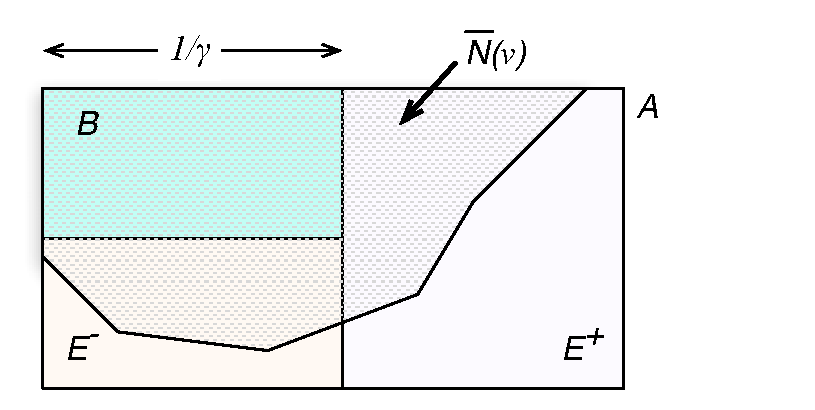
\includegraphics[width=3.2in]{./FIGURES/proof_of_lemma_PD'3a.pdf}
\caption{Illustration of the sets $\wbarN(\nu)$, $A$, $B$,
  $E^-$ and $E^+$ in the proof of Lemma~\ref{lem: PD1:
    primary overlap}. We have $A=\wtildeN(j), B =
  \wtildeclsnb(j) \cap \wbarclsnb(\kappa), E^- =
  \wtildeclsnb(j) - \wbarclsnb(\kappa), E^+ = \wtildeN(j) -
  \wtildeclsnb(j)$.}
\label{fig: sets lemma PD'3a}
\end{center}
\end{figure}

  We define the sets $A$, $B$, $E^-$ and $E^+$ as the subsets of
  $\facilityset$ (the final set of facilities) that were obtained from
  splitting facilities in the sets $\wtildeN(j)$, $\wtildeclsnb(j)\cap
  \wbarclsnb(\kappa)$, $\wtildeclsnb(j) - \wbarclsnb(\kappa)$ and
  $\wtildeN(j) - \wtildeclsnb(j)$, respectively.  (See
  Figure~\ref{fig: sets lemma PD'3a}.)  We claim that at the end
  $B\subseteq \wbarclsnb(\nu)$, with the caveat that the ties in the
  definition of $\wbarclsnb(\nu)$ are broken in favor of the
  facilities in $B$.  (This is the tie-breaking rule that we mentioned
  in the definition of $\wbarclsnb(\nu)$.)  This will be sufficient to
  prove the lemma because $B\neq\emptyset$, by the algorithm.

  We now prove this claim. Note first that $B\subseteq \wbarN(\nu)
  \subseteq A$, because we never remove facilities from $\wbarN(\nu)$
  and we only add facilities from $\wtildeN(j)$.  Also, $B\cup E^-$
  represents the facilities obtained from $\wtildeclsnb(j)$, so
  $\sum_{\mu\in B\cup E^-} \bary_{\mu} = 1/\gamma$.  This and
  $B\subseteq \wbarN(\nu)$ implies that the total connection value of
  $B\cup (\wbarN(\nu)\cap E^-)$ to $\nu$ is at most $1/\gamma$. But
  all facilities in $B\cup (\wbarN(\nu)\cap E^-)$ are closer to $\nu$
  than those in $E^+\cap \wbarN(\nu)$. It follows that $B\subseteq
  \wbarclsnb(\nu)$, completing the proof.
\end{proof}

%%%%%%%%%%%%%%

\begin{lemma}\label{lem: PD1: primary optimal}
  Property (PD'.\ref{PD:assign:cost}) holds.
\end{lemma}

\begin{proof}
This proof is similar to that for Lemma~\ref{lem: PD:assign:cost holds}.
For a client $j$ and demand $\eta$, we will write
$\tcccls^\eta(j)$ and $\dmaxcls^\eta(j)$ to denote the values of
$\tcccls(j)$ and $\dmaxcls(j)$ at the time when $\eta$
was created. (Here $\eta$ may or may not be a demand of client $j$).

Suppose $\nu \in j$ is assigned to a primary demand $\kappa \in p$.
By the way primary demands are constructed in the partitioning
algorithm, $\wtildeclsnb(p)$ becomes $\wbarclsnb(\kappa)$, so we have
$\clsdist(\kappa) = \tcccls^\kappa (p)$ and $\clsmax(\kappa) =
\tcccls^\kappa(p)$. Further, since we choose $p$ to minimize
$\tcccls(p) + \dmaxcls(p)$, we thus have that $\tcccls^\kappa(p) +
\dmaxcls^\kappa(p) \leq \tcccls^\kappa(j) + \dmaxcls^\kappa(j)$ at the
time when demand $\kappa$ was created.

Using an argument analogous to that in the proof of Lemma~\ref{lem: tcc optimal}, 
our modified partitioning algorithm guarantees that
  $\tcccls^{\kappa}(j) \leq \tcccls^{\nu}(j)$ and
  $\dmaxcls^{\kappa}(j) \leq \dmaxcls^{\nu}(j)$ since $\nu$ was
  created later.
  Therefore, we have
%
  \begin{align*}
    \clsdist(\kappa) + \clsmax(\kappa) &= \tcccls^{\kappa}(p) +	\dmaxcls^{\kappa}(p) 
					\\
					&\leq \tcccls^{\kappa}(j) + \dmaxcls^{\kappa}(j) 
					\leq \tcccls^{\nu}(j) + \dmaxcls^{\nu}(j) 
					= \clsdist(\nu) + \clsmax(\nu),
  \end{align*}
%
completing the proof.
\end{proof}

%%%%%%%%

Now we have completed the proof that the computed partitioning satisfies
all the required properties. 


\paragraph{Algorithm~{\EBGS}.}
The complete algorithm starts with solving the linear program and
computing the partitioning described earlier in this section.  Given
the partitioned fractional solution $(\barbfx, \barbfy)$ with the
desired properties, we start the process of opening facilities and
making connections to obtain an integral solution. To this end, for
each primary demand $\kappa\in P$, we open exactly one facility
$\phi(\kappa)$ in $\wbarclsnb(\kappa)$, where each
$\mu\in\wbarclsnb(\kappa)$ is chosen as $\phi(\kappa)$ with
probability $\gamma\bary_{\mu}$. For all facilities
$\mu\in\facilityset - \bigcup_{\kappa\in P}\wbarclsnb(\kappa)$, we
open them independently, each with probability
$\gamma\bary_{\mu}$. Due to our choice of $\gamma$ being $1 < \gamma <
2$, we have $1-1/\gamma \leq 1/\gamma$ so property (CO) actually
implies all $\bary_{\mu} \leq 1/\gamma$ since there exists some $\nu$
such that $\barx_{\mu\nu} = \bary_{\mu}$ and any
$\mu\in\wbarclsnb(\nu)$ satisfies $\barx_{\mu\nu} \leq 1/\gamma$, and
any $\mu\in\wbarfarnb(\nu)$ satisfies $\barx_{\mu\nu} \leq
1-1/\gamma$. Then all $\gamma\bary_{\mu}$ are valid probablity values.

Next, we connect demands to facilities.
Each primary demand $\kappa\in P$ will connect
to the only open facility $\phi(\kappa)$ in $\wbarclsnb(\kappa)$.  
For each non-primary demand $\nu\in \demandset - P$, if
there is an open facility in $\wbarN(\nu)$ then we connect
$\nu$ to the nearest such facility. Otherwise, we connect
$\nu$ to its \emph{target facility} $\phi(\kappa)$, where $\kappa$ is the primary
demand that $\nu$ is assigned to. 

%%%%%%%%%%%

\paragraph{Analysis.}
By the algorithm, for each client $j$, all its $r_j$ demands are connected to
open facilities. If two different siblings $\nu,\nu'\in j$ are assigned, respectively,
to primary demands $\kappa$, $\kappa'$ then, by
Properties~(SI'.\ref{SI1:siblings disjoint}), (SI'.\ref{SI1:primary
  disjoint}), and (PD'.\ref{PD1:disjoint}) we have
%
\begin{equation*}
( \wbarN(\nu) \cup \wbarclsnb(\kappa)) \cap (\wbarN(\nu')\cup \wbarclsnb(\kappa')) = \emptyset.
\end{equation*}
%
This condition guarantees that $\nu$ and $\nu'$ are assigned to different facilities,
regardless whether they are connected to a neighbor facility or to its target facility.
Therefore the computed solution is feasible.

\smallskip

We now estimate the cost of the solution computed by Algorithm {\EBGS}. The lemma
below bounds the expected facility cost.

\begin{lemma} \label{lem: EBGS facility cost}
The expected facility cost $F_{\smallEBGS}$ of Algorithm~{\EBGS} is at most $\gamma F^\ast$.
\end{lemma}

\begin{proof}
By the algorithm, each facility $\mu\in \facilityset$ is opened with
probability $\gamma \bary_{\mu}$, independently of whether it belongs to the
close neighborhood of a primary demand or not. Therefore, by
  linearity of expectation, we have that the expected facility cost is
%
\begin{equation*}
	F_{\smallEBGS} = \sum_{\mu \in \facilityset} f_\mu \gamma \bary_{\mu} 
			= \gamma \sum_{i\in \sitesset} f_i \sum_{\mu\in i} \bary_{\mu} 
			\stackrel{\ast}{=} \gamma \sum_{i \in \sitesset} f_i y_i^\ast = \gamma F^\ast,
\end{equation*}
%
where the $(\ast)$ equality follows from (PS.\ref{PS:yi}).
\end{proof}

%%%%%%%%%%%

To bound the connection cost, we start with a lemma that
estimates the cost of indirect connections, between a
non-primary demand and its target facility. The proof of
this lemma relies on
Properties~(PD'.\ref{PD1:assign:overlap}) and
(PD'.\ref{PD1:assign:cost}) of modified partitioning and
follows the reasoning in the proof of a similar lemma
in~\cite{ByrkaGS10,ByrkaA10}.  For the sake of completeness,
we include a proof is in the appendix.

\begin{lemma}\label{lem: EBGS target connection cost}
  In Algorithm~{\EBGS}, let $\gamma$ be a constant such that $1 <
  \gamma < 2$, for a non-primary demand $\nu$, in the event that no
  facility in $\wbarN(\nu)$ opens, the expected connection cost is no
  more than $\clsdist(\nu)+\clsmax(\nu)+\fardist(\nu)$.
\end{lemma}

We are now ready to bound the overall connection cost of Algorithm~{\EBGS}.

\begin{lemma}\label{lem: EBGS connection cost}
  Assuming that $1 < \gamma < 2$, the expected connection
  cost $C_{\smallEBGS}$ of Algorithm~{\EBGS} is at most
  $C^\ast\cdot\max\{\frac{1/e+1/e^\gamma}{1-1/\gamma},
  1+\frac{2}{e^\gamma}\}$.
\end{lemma}

\begin{proof}
  The argument is similar to that in~\cite{ByrkaGS10}. Fix some
  non-primary demand $\nu$. Let $\wbarclsnb(\nu) =
  \{\mu_1,\ldots,\mu_l\}$ and $\wbarfarnb(\nu) = \{\mu_{l+1}, \ldots,
  \mu_{l'}\}$, where facilities are ordered by non-decreasing distance
  to $\nu$, and $d_1,\ldots,d_l,d_{l+1},\ldots,d_{l'}$ be the
  corresponding distance to $\nu$. Let $\Lambda_{\nu}$ be the event
  that none of $\wbarN(\nu)$ opens in algorithm {\EBGS}'s integral
  solution and $\kappa$ be the primary demand that $\nu$ was assigned
  to, we then have $\Exp[d_{\phi(\kappa)\nu}\mid \Lambda_{\nu}] \leq
  \clsdist(\nu) + \clsmax(\nu) + \fardist(\nu)$ by Lemma~\ref{lem:
    EBGS target connection cost}.

  Let $C_{\nu}$ be the random variable of the distance from
  $\nu$ to the facility that it connects to in the integral
  solution. A similar argument to estimate the distance by a
  provably worse random process, as in the analysis of
  algorithm {\ECHS}, will then show that the expected
  distance $\Exp[C_\nu]$ is no more than the estimate that
  uses the nearest facility in $\wbarclsnb(\nu)$ if one
  opened, then use the nearest in $\wbarfarnb(\nu)$ if there
  is one, and only use $\phi(\kappa)$ if none in
  $\wbarN(\nu)$ opened. A detailed derivation follows.
  \begin{align*}
    \Exp[C_{\nu}] 
    &\leq \left(1-\prod_{s=1}^l (1-\gamma\bary_s)\right) \sum_{s=1}^l d_s \gamma\bary_s\\
    &+ \left(\prod_{s=1}^l(1-\gamma\bary_s) - \prod_{s=1}^{l'}(1-\gamma\bary_s)\right) \left(\sum_{s=l+1}^{l'} d_s\bary_s\;/ \;\sum_{s=l+1}^{l'} \bary_s \right)\\
    &+ \left(\prod_{s=1}^{l'} (1-\gamma\bary_s)\right) \Exp[d_{\phi(\kappa)\nu} \mid \Lambda_\nu]\\
    &\leq (1-1/e)\clsdist(\nu) + (1/e - 1/e^\gamma)\fardist(\nu) + 1/e^\gamma (\clsdist(\nu) + \clsmax(\nu) + \fardist(\nu))\\
\\
  &\leq 
	\textstyle
	\clsdist(\nu)(1-\frac{1}{e}) + \fardist(\nu)(\frac{1}{e}-\frac{1}{e^\gamma})
	 			+ (\clsdist(\nu)+2\fardist(\nu))\frac{1}{e^\gamma}
\\
  &\leq
	\textstyle
  \concost(\nu)((1-\rho_{\nu})(\frac{1/e+1/e^\gamma}{1-1/\gamma})
  + \rho_{\nu}(1+\frac{2}{e^\gamma}) 
\\
  &\leq 
	\textstyle
	\concost(\nu) \cdot \max\Big\{\frac{1/e+1/e^\gamma}{1-1/\gamma},
  								1+\frac{2}{e^\gamma}\Big\},
\end{align*}
%
where $\rho_{\nu}=\clsdist(\nu)/\concost(\nu)$. It is easy to see that
$\rho_{\nu}$ is between 0 and 1. In the second inequality we used the
fact that $\sum_{s=1}^l \bary_{s} = 1/\gamma$ and $\sum_{s=1}^{l'}
\bary_{s} = 1$. Since $\sum_{\nu\in j} C^{\avg}(\nu)
= \sum_{\nu\in j}\sum_{\mu\in\facilityset} d_{\mu\nu}\barx_{\mu\nu} =
\sum_{i\in\sitesset} d_{ij}x_{ij}^\ast = C_j^\ast$, summing over all
clients $j$ we have total connection cost bounded by \\$C^\ast
\max\{\frac{1/e+1/e^\gamma}{1-1/\gamma}, 1+\frac{2}{e^\gamma}\}$.
\end{proof}

Recall that the expected facility cost is bounded by $\gamma F^\ast$,
as argued earlier. Hence the total cost is bounded by $\max\{\gamma,
\frac{1/e+1/e^\gamma}{1-1/\gamma}, 1+\frac{2}{e^\gamma}\}\cdot
\LP^\ast$. Picking $\gamma=1.575$ we obtain the desired ratio.


\begin{theorem}\label{thm:ebgs}
  Algorithm~{\EBGS} is a $1.575$-approximation algorithm for \FTFP.
\end{theorem}





%%%%%%%%%%%%%%%%%%%%%%

\section{Final Comments}

In this paper we show a sequence of LP-rounding approximation algorithms
for FTFP, with the best algorithm achieving  ratio $1.575$. 
As we mentioned earlier, we believe that 
our techniques of demand reduction and adaptive partitioning are very flexible and
should be useful in extending other LP-rounding methods for UFL to obtain
matching bounds for FTFP.

One of the main open problems in this area is whether FTFL can be approximated with the
same ratio as UFL, and our work was partly motivated by this question. The techniques we
introduced are not directly applicable to FTFL, mainly because our partitioning
approach involves facility splitting that could result in several sibling demands being served
by facilities on the same site. Nonetheless, we hope that further refinements of 
our construction might get around this issue and
lead to new algorithms for FTFL with improved ratios.
\pagebreak

\bibliographystyle{elsarticle-num}
\bibliography{facility}

\pagebreak
%%%%%%%%%%%%%%%%%%%%%%%%%%%%%%%%%%%%%%%%%%%%%%%%%%%%%%%%%%%%%%%%%%%%%%%%%%%%%%%%
%%%%%%%%%%%%%%%%%%%%%%%%%%%%%%%%%%%%%%%%%%%%%%%%%%%%%%%%%%%%%%%%%%%%%%%%%%%%%%%%
%%%%%%%%%%%%%%%%%%%%%%%%%%%%%%%%%%%%%%%%%%%%%%%%%%%%%%%%%%%%%%%%%%%%%%%%%%%%%%%%

\appendix
\section{Proof of Lemma~\ref{lem: EBGS target connection cost}}
  Lemma~\ref{lem: EBGS target connection cost} provides a bound on the
  expected connection cost of a demand $\nu$ when none of
  $\wbarN(\nu)$ opens by the algorithm. The formal proof is very
  similar to that in \cite{ByrkaA10}, and we sketch the main steps
  here for completeness.

  Let $K_1 = \wbarclsnb(\kappa) \setminus \wbarN(\nu), K_2 =
  \wbarclsnb(\kappa) \cap \wbarclsnb(\nu)$ and $K_3 =
  \wbarclsnb(\kappa) \cap \wbarfarnb(\nu)$, then we shall show that
  $D(K_1, \nu) \leq \clsdist(\kappa)+\clsmax(\kappa) + 
  \fardist(\nu)$, which implies $D(K_1, \nu) \leq \clsdist(\nu) +
  \clsmax(\nu) + \fardist(\nu)$ due to
  (PD'.\ref{PD1:assign:cost}). Recall that $D(A,\nu)
  \stackrel{\mathrm{def}}{=} \sum_{\mu\in A} d_{\mu\nu}\bary_{\mu}$ is
  the average distance of facilities in set $A$ to demand $\nu$.

  We can dismiss a few simple cases: If $D(K_1, \kappa) \leq
  \clsdist(\kappa)$, then we can use any facility $\mu \in K_2$ to
  show that $D(K_1,\nu) \leq D(K_1, \kappa) + d_{\mu\kappa} +
  d_{\mu\nu} \leq \clsdist(\kappa) + \clsmax(\kappa) + \fardist(\nu)$
  because $d_{\mu\kappa} \leq \clsmax(\kappa)$ and $d_{\mu\nu} \leq
  \clsmax(\nu) \leq \fardist(\nu)$, and we are done. So we can assume
  $D(K_1, \kappa) > \clsdist(\kappa)$. Our second assumption is that
  every $\mu \in K_2$ has $d_{\mu\kappa} > \clsdist(\kappa)$, for
  otherwise we can use $\clsmax(\kappa)$ to bound $D(K_1, \kappa)$ and
  there exists a facility $\mu\in K_2$ such that $d_{\mu\kappa} \leq
  \clsdist(\kappa)$. Since $\mu\in K_2$, we infer that $d_{\mu\nu}
  \leq \clsmax(\nu) \leq \fardist(\nu)$, and we are done as well.

  Given the two assumptions we can now assume that $K_3$ is not empty
  and there exists some finite number $\delta > 0$ such that $D(K_3,
  \kappa) = \clsdist(\kappa) - \delta$. This in turn implies $D(K_3,
  \nu) \geq \fardist(\nu) + \delta$, or we will be done. Because $K_3$
  is a subset of $\wbarfarnb(\nu)$, this gives us a bound on
  $D(\wbarfarnb(\nu) \setminus K_3, \nu)$, which in turn, is an upper
  bound on $\clsmax(\nu)$. Let $\hat{y} = \gamma \sum_{\mu\in K_3}
  \bary_{\mu}$, using the fact that $\fardist(\nu) = D(K_3,\nu)\;
  \hat{y}/(\gamma-1) + D(\wbarfarnb(\nu)\setminus K_3)\;
  (\gamma-1-\hat{y})/(\gamma-1)$, we are able to show that
  \begin{equation*}
    \clsmax(\nu) \leq D(\wbarfarnb(\nu) \setminus K_3, \nu) \leq \fardist(\nu) -
    \hat{y}\delta/(\gamma-1-\hat{y}) \leq \fardist(\nu) -
    \hat{y}\delta/(1-\hat{y}),
  \end{equation*}
  since $\gamma \leq 2$ (we pick $\gamma=1.575$ in the end). On the
  other hand, since $\wbarclsnb(\kappa) = K_1 \cup K_2 \cup K_3$, we
  have $\clsdist(\kappa) = (1-\hat{y})\; D(K_1\cup K_2, \kappa) +
  \hat{y}\; D(K_3, \kappa)$, which implies that
  \begin{equation*}
    D(K_1 \cup K_2, \kappa) = \clsdist(\kappa) + \hat{y}\delta/(1-\hat{y}).
  \end{equation*}

  Now we are essentially done. If there exists some $\mu \in K_2$ such
  that $d_{\mu\kappa} \leq \clsdist(\kappa) +
  \hat{y}\delta/(1-\hat{y})$, then we have
  \begin{align*}
    D(K_1, \nu) &\leq D(K_1, \kappa) + d_{\mu\kappa} + d_{\mu\nu} \\
    &\leq \clsmax(\kappa) + \clsdist(\kappa) +
    \hat{y}\delta/(1-\hat{y})
    + \clsmax(\nu)\\
    &\leq \clsmax(\kappa) + \clsdist(\kappa) + \fardist(\nu)
  \end{align*}
  Otherwise we must have $D(K_1, \kappa) \leq \clsdist(\kappa) +
  \hat{y}\delta/(1-\hat{y})$. It follows that
  \begin{align*}
    D(K_1, \nu) &\leq D(K_1, \kappa) + d_{\mu\kappa} + d_{\mu\nu} \\
    &\leq \clsdist(\kappa) + \hat{y}\delta/(1-\hat{y}) +
    \clsmax(\kappa)
    + \clsmax(\nu)\\
    &\leq \clsmax(\kappa) + \clsdist(\kappa) + \fardist(\nu).
  \end{align*}

  This concludes the proof of Lemma~\ref{lem: EBGS target connection
    cost}, and we have the desired bound on the expected distance when
  the algorithm connnects a demand $\nu$ indirectly to its target
  facility, that is, the facility opened by the primary demand that
  $\nu$ was assigned.


%%%%%%%%%%%%%%%%%%%%%%%%%%%%%%%%%%%%%%%%%%%%%%%%%%%%%%%%%%%%%%%%%%%%
%%%%%%%%%%%%%%%%%%%%%%%%%%%%%%%%%%%%%%%%%%%%%%%%%%%%%%%%%%%%%%%%%%%%
%%%%%%%%%%%%%%%%%%%%%%%%%%%%%%%%%%%%%%%%%%%%%%%%%%%%%%%%%%%%%%%%%%%%

\section{Proof of an Inequality for Analysis of Algorithm~{\ECHS}}

In the $1+2/e=1.736$-approximation in Section~\ref{sec: 1.736-approximation}
we need to show the following inequality
%
\begin{equation}
  \label{eq:dist}
\sum_{u=1}^l d_uy_u\prod_{s=1}^{u-1}(1-y_s)
  \;\leq\;  \Big(1 - \prod_{s=1}^l (1-y_s)\Big) \cdot \sum_{u=1}^l d_u y_u
\end{equation}
%
for $d_1\leq d_2 \leq \ldots \leq d_l$ and $\sum_{s=1}^l y_s = 1, y_s \geq 0$.

In this section we give a new proof of this inequality, much
simpler than the existing proof in \cite{ChudakS04}, and also simpler than
the argument by Sviridenko~\cite{Svi02}.  
We derive this inequality from the following generalized version of the Chebyshev Sum
Inequality:
%
\begin{equation}
  \label{eq:cheby}
  \sum_{i} p_i \sum_j p_j a_j b_j \leq \sum_i p_i a_i \sum_j p_j b_j,
\end{equation}
%
where each summation below runs from $1$ to $l$ and the sequences 
$(a_i)$, $(b_i)$ and $(p_i)$ satisfy the following conditions:
$p_i\geq 0, a_i \geq 0, b_i \geq 0$ for all $i$, $a_1\leq a_2 \leq
\ldots \leq a_l$, and $b_1 \geq b_2 \geq \ldots \geq b_l$.

Given inequality (\ref{eq:cheby}), we can obtain our inequality
(\ref{eq:dist}) by simple substitution
%
\begin{equation*}
  p_i \leftarrow y_i, a_i \leftarrow d_i, b_i \leftarrow
  \Pi_{s=1}^{i-1} (1-y_s).
\end{equation*}

For the sake of completeness, we include the proof of inequality (\ref{eq:cheby}), 
due to Hardy, Littlewood and Polya~\cite{HardyLP88}. The idea is to evaluate the 
following sum:
%
\begin{align*}
  S &= \sum_i p_i \sum_j p_j a_j b_j - \sum_i p_i a_i \sum_j p_j b_j
	\\
  & = \sum_i \sum_j p_i p_j a_j b_j - \sum_i \sum_j p_i a_i p_j b_j
	\\
  & = \sum_j \sum_i p_j p_i a_i b_i - \sum_j \sum _i p_j a_j p_i b_i
	\\
	&= \half \cdot \sum_i \sum_j (p_i p_j a_j b_j - p_i a_i p_j b_j + p_j p_i a_i
  							b_i - p_j a_j p_i b_i)
\\
  &= \half \cdot \sum_i \sum_j p_i p_j (a_i - a_j)(b_i - b_j) \leq 0.
\end{align*}
The last inequality holds because $(a_i-a_j)(b_i-b_j) \leq 0$, since the sequences
$(a_i)$ and $(b_i)$ are ordered oppositely.

\end{document}

% marek Tue Jul  3 10:21:05 PDT 2012
% marek Sun Jul  1 14:57:39 PDT 2012
% lyan Sat Jun 30 2012, 22:01:27
% marek Sat Jun 30 10:08:59 PDT 2012
% lyan Fri Jun 29 19:54:18 PDT 2012
% marek Thu Jun 28 09:21:14 PDT 2012
% lyan Thu Jun 28 00:11:28 PDT 2012
% marek Wed Jun 27 11:24:07 PDT 2012
% lyan Wed Jun 27 2012, 10:08:21
% marek Tue Jun 26 14:48:45 PDT 2012
% lyan Mon Jun 25 2012, 22:23:13
% marek Sun Jun 24 16:46:23 PDT 2012
% marek Wed Jun 20 04:42:40 PDT 2012
% lyan, Sun Jun 17 2012, 09:49:22
% marek Sat Apr  7 16:42:21 PDT 2012
% marek Thu Apr  5 11:39:58 PDT 2012
% marek Wed Apr  4 11:28:20 PDT 2012
% lyan, 04/01/12 10:20 PM
% lyan, Mon Mar 26 2012, 09:10:54
% lyan, Tue Mar 20 2012, 23:28:17
% lyan, 03/18/12 12:28 PM
% marek Sat Mar 17 13:42:32 PDT 2012
% marek, Wed Mar  7 21:28:24 PST 2012
% marek Mon Mar 12 12:08:25 PDT 2012
